\chapter{VIC-IV Video Interface Controller}
\label{cha:viciv}

\section{Kenmerken}De VIC-IV is een vierde generatie Video Interface Controller die speciaal voor de MEGA65 is ontwikkeld en beschikt over een zeer goede backwards compatibility met de VIC-II die in de C64 werd gebruikt en de VIC-III die in de C65 werd gebruikt. De VIC-IV kan geprogrammeerd worden alsof het een van deze voorgangersystemen betreft. Daarnaast ondersteunt het een aantal nieuwe functies. Het is eenvoudig om oudere VIC-II/III-functies te combineren met de nieuwe VIC-IV-functies, waardoor de overstap van de VIC-II of VIC-III naar de VIC-IV net zo eenvoudig is als de overstap van de VIC-II naar de VIC-III destijds. Enkele van de nieuwe functies en verbeteringen van de VIC-IV zijn:

\begin{itemize}
\item {\bf Directe toegang tot 384KB RAM} (ten opzichte van 16KB/64KB met de VIC-II en 128KB met de VIC-III).\item Ondersteuning voor {\bf 32KB 8-bits kleuren-/attribuutgeheugen} (ten opzichte van 2KB op de VIC-III), om zeer grote schermen te ondersteunen.\item {\bf HDTV 720$\times$576 / 800$\times$600 native resolutie} bij zowel 50 Hz als 60 Hz voor {\bf PAL en NTSC}, met {\bf VGA en digitale video}uitvoer.\item {\bf 81 MHz pixelklok} (ten opzichte van $\sim$ 8 MHz met de VIC-II/III), waardoor een breed scala aan nieuwe functies mogelijk wordt.\item Nieuwe 16-kleuren (16$\times$8 pixels per tekencel) en 256-kleuren (8$\times$8 pixels per tekencel) {\bf volkleur-tekstmodi}.\item Ondersteuning voor maximaal {\bf 8.192 unieke tekens in een tekenset}.\item {\bf Vier 256-kleuren paletbanken} (ten opzichte van de enkele paletbank van de VIC-III), die elk een {\bf 23-bits kleurdiepte} ondersteunen (ten opzichte van de 12-bits kleurdiepte van de VIC-III) en die snel kunnen worden gewisseld om nog kleurrijkere afbeeldingen te produceren dan mogelijk is met de VIC-III.\item Scherm-, bitmap-, kleur- en tekengegevens kunnen op elk {\bf adres met byte-nauwkeurigheid} worden gepositioneerd (in tegenstelling tot de vaste 1KB -- 16KB-grenzen van de VIC-II/III).\item {\bf Virtuele schermafmetingen}, die gecombineerd met byte-nauwkeurige gegevensposities {\bf hardware-ondersteuning voor scrollen en pannen in zowel X- als Y-richting} bieden.\item {\bf Nieuwe sprite-modi}: bitplanewijziging, {\bf volkleuren} (15 voorgrondkleuren + transparantie) en getegelde modi, die een breed scala aan nieuwe en spannende sprite-gebaseerde effecten mogelijk maken.\item De mogelijkheid om sprites stapelvormig in bitplane-vorm te rangschikken om {\bf sprites met maximaal 256 kleuren} te produceren.\item Sprites kunnen 64 bits gegevens per rasterlijn gebruiken, waardoor {\bf sprites 64 pixels breed} kunnen zijn bij gebruik van de VIC-II/III mono-/multicolour-modus, of 16 pixels breed bij gebruik van de nieuwe VIC-IV volkleur-spritemodus.\item {\bf Sprite-tegelmodus}, waarmee een sprite horizontaal kan worden herhaald over de volledige rasterlijn, waardoor sprites kunnen worden gebruikt om geanimeerde achtergronden te creëren op een geheugenefficiënte manier.\item Sprites kunnen worden geconfigureerd om een {\bf apart 256-kleurenpalet} te gebruiken in plaats van het palet dat voor andere tekst en afbeeldingen wordt gebruikt, waardoor een kleurrijker beeld mogelijk is.\item {\bf Super-uitgebreide attribuutmodus} die per tekenmodus twee schermgeheugenbytes en twee kleurengeheugenbytes gebruikt en een breed scala aan nieuwe functies ondersteunt, waaronder {\bf alfa-menging/anti-aliasing}, {\bf hardware-kerning/letters met variabele breedte}, hardwarematig horizontaal/verticaal spiegelen, selectie van een alternatief palet en andere krachtige functies die het gemakkelijk maken om zeer dynamische en kleurrijke weergaven te creëren.\item {\bf Raster-Rewrite Buffer} waarmee {\bf hardwarematig gegenereerde pseudo-sprites} mogelijk zijn, vergelijkbaar met ``bobs'' op Amiga\texttrademark{}-computers, maar met het voordeel dat ze in de weergavepijplijn worden gerenderd en dus niet hoeven te worden gewist en opnieuw getekend om te animeren.\item Ook {\bf verschillende 8-bits kleuren-playfields} zijn mogelijk via de Raster-Rewrite Buffer.
\end{itemize}

Kortom, de VIC-IV is een krachtige evolutie van de VIC-II/III, waarbij het karakter en de eigenaardigheden van de VIC-reeks videocontrollers behouden zijn gebleven.

Voor een volledige beschrijving van de extra registers die de VIC-IV biedt, alsmede documentatie van de legacy VIC-II- en VIC-III-registers, verwijst u naar de betreffende secties van deze bijlage. Het resterende deel van de bijlage richt zich op het beschrijven van de mogelijkheden en het gebruik van veel van de nieuwe functies van de VIC-IV.


\section{Toegang tot VIC-III/IV-registers}Omdat de nieuwe functies van de VIC-IV allemaal uitbreidingen zijn op de bestaande VIC-II/III-ontwerpen, bestaat er geen concept van het moeten selecteren van de modus waarin de VIC-IV zal werken: deze bevindt zich altijd in VIC-IV-modus. Voor backwards compatibility met software kunnen de vele extra registers van de VIC-IV echter verborgen worden, zodat de VIC-IV zich voordoet als een VIC-II of VIC-III. Dit gebeurt op dezelfde wijze als waarop de VIC-III zijn nieuwe functies verbergt voor legacy VIC-II-software.

 Het mechanisme is het write-only KEY-register van de VIC-III (\$D02F, 53295 decimaal). De VIC-III verbergt standaard zijn nieuwe functies totdat een ``klop''-sequentie wordt uitgevoerd. Deze bestaat uit het achtereenvolgens schrijven van twee speciale waarden naar \$D02F. De volgende samenvattende tabel toont de ondersteunde klopsequenties van de VIC-IV en geeft aan welke VIC-IV-specifiek zijn en welke ook door de VIC-III worden ondersteund:

\setlength{\tabcolsep}{3pt}
{\small \begin{longtable}{|L{2.4cm}|L{2.4cm}|L{3.9cm}|L{1.6cm}|}
\hline
{\bf{Eerste waarde Hex (Decimaal)}} & {\bf{Tweede waarde Hex (Decimaal)}} & {\bf{Effect}} & {\bf{VIC-IV-specifiek? }} \\
\hline
\endfirsthead
\multicolumn{3}{l@{}}{\ldots Vervolgd}\\
\hline
{\bf{Eerste waarde Hex (Decimaal)}} & {\bf{Tweede waarde Hex (Decimaal)}} & {\bf{Effect}} & {\bf{VIC-IV-specifiek? }} \\
\hline
\endhead
\multicolumn{3}{l@{}}{Vervolgd \ldots}\\
 \endfoot
 \hline
\endlastfoot
\small \$00 (0) & \small \$00 (0) & Alleen VIC-II-re\-gis\-ters zichtbaar (alle nieuwe VIC-III- en VIC-IV-re\-gis\-ters zijn verborgen) & Nee \\
 \hline
\small \$A5 (165) & \small \$96 (150) & Nieuwe VIC-III-re\-gis\-ters zichtbaar & Nee \\
 \hline
\small \$47 (71) & \small \$53 (83) & Zowel nieuwe VIC-III- als VIC-IV-re\-gis\-ters zichtbaar & Ja \\
 \hline
\small \$45 (69)  & \small \$54 (84) & Geen VIC-II/III/IV-re\-gis\-ters zichtbaar. In plaats daarvan zijn de buffers van de 45E100-Ether\-net\-con\-trol\-ler zichtbaar & Ja \\
 \hline
   \end{longtable}}


 \subsection{VIC-II/III/IV detecteren}

 Het bepalen van welke generatie VIC-II/III/IV in een computer is geïnstalleerd, kan belangrijk zijn voor programma's die slechts bepaalde generaties ondersteunen of die hun grafische weergave willen laten variëren op basis van de mogelijkheden van de computer. Hoewel er hiervoor veel mogelijkheden bestaan, volgt hier een eenvoudige en effectieve methode. Deze berust op het feit dat de VIC-III en VIC-IV de VIC-II-registers niet door de hele I/O-adresruimte herhalen. Terwijl \$D000 en \$D100 synoniem zijn wanneer een VIC-II aanwezig is (of een VIC-III/IV zijn extra registers verbergt), is dit niet het geval wanneer een VIC-III of VIC-IV alle registers zichtbaar maakt. De aanwezigheid van een VIC-III/IV kan daarom worden vastgesteld door te testen of deze twee locaties aliasen zijn van hetzelfde register of afzonderlijke registers vertegenwoordigen. De detectiesequentie bestaat uit het gebruik van het KEY-register om extra VIC-IV- of VIC-III-registers zichtbaar te maken. Indien een van beide lukt, kan worden aangenomen dat de overeenkomstige VIC-generatie is geïnstalleerd. Omdat de VIC-IV de VIC-III-klopsequenties ondersteunt, moet eerst op de aanwezigheid van een VIC-IV worden getest. Tevens gaan we ervan uit dat de MEGA65 in VIC-IV-modus start, zelfs wanneer C65 BASIC wordt uitgevoerd. De test kan daarom vanuit BASIC worden uitgevoerd, zowel vanuit C64- als C65-modus als volgt:

\begin{screencode}
0 REM IN C65-MODUS KUNNEN WE NIET VEILIG NAAR $D02F SCHRIJVEN,
1 REM DUS TESTEN WE HET OP EEN ANDERE MANIER
10 IF PEEK($D018) AND 32 THEN GOTO 65
20 POKE $D000,1:POKE $D02F,71:POKE $D02F,83
30 POKE $D000+256,0:IF PEEK($D000)=1 THEN PRINT"VIC-IV AANWEZIG":END
40 POKE $D000,1:POKE $D02F,165:POKE $D02F,150
50 POKE $D000+256,0:IF PEEK($D000)=1 THEN PRINT"VIC-III AANWEZIG":END
60 PRINT "VIC-II AANWEZIG":END
65 REM WE GAAN ERVAN UIT DAT WE HIER EEN C65 HEBBEN
70 V1=PEEK($D050):V2=PEEK($D050):V3=PEEK($D050)
80 IF V1<>V2 OR V1<>V3 OR V2<>V3 THEN PRINT "VIC-IV PRESENT":END
90 GOTO 40
\end{screencode}

Regel 10 van dit programma controleert of het scherm een veelvoud van 2KB is. Omdat het scherm op de C64 op 1KB staat, slaagt deze test niet en gaat de uitvoering verder naar regel 20. Regel 20 schrijft 1 naar een van de VIC-II-spritepositieregisters, 53248, en vervolgens de MEGA65-klop naar het KEY-register, 53295. Regel 30 schrijft naar 53248 + 256, wat op de C64 een spiegel is van 53248, maar op een MEGA65 met VIC-IV I/O ingeschakeld een van de rode paletregisters is. Na het schrijven naar 53248 + 256 controleert het programma of het register op 53248 is gewijzigd door de schrijfactie naar 53248 + 256. Indien dat het geval is, verwijzen de twee adressen naar hetzelfde register. Dit gebeurt op zowel een C64 als een C65, maar niet op een computer met een VIC-IV. Wanneer 53248 dus niet is gewijzigd, melden we dat we een VIC-IV hebben gedetecteerd. Indien het schrijven naar 53248 + 256 de waarde in register 53248 wel heeft gewijzigd, gaat het programma verder naar regel 40, die opnieuw naar 53248 schrijft en ditmaal de VIC-III-klop naar het KEY-register schrijft. Regel 50 is gelijk aan regel 30, maar omdat deze na een VIC-III-klop verschijnt, maakt ze de detectie van een VIC-III mogelijk. Indien ten slotte noch een VIC-IV noch een VIC-III wordt gedetecteerd, concluderen we dat er alleen een VIC-II aanwezig moet zijn.

Omdat de MEGA65 de enige C64-klassecomputer is die over een VIC-IV beschikt, kan dit als een {\em de facto}-test voor de aanwezigheid van een MEGA65-computer worden gebruikt. Detectie van een VIC-III kan op vergelijkbare wijze worden aangenomen dat deze de aanwezigheid van een C65 aanduidt.

\section{Video-uitvoerformaten, timing en compatibiliteit}

 \subsection{Integrated Marvellous Digital Hookup\texttrademark{} (IMDH\texttrademark{})  Digitale video-uitvoer}
  \index{Integrated Marvellous Digital Hookup\texttrademark}
  \index{IMDH\texttrademark}

De MEGA65 beschikt over VGA-analoge video-uitvoer en Integrated Marvellous Digital Hookup\texttrademark{} (IMDH\texttrademark{}). Dit wijkt in een aantal opzichten af van bestaande gangbare digitale videostandaarden:

\begin{enumerate}
  \item We hebben er geen nieuwe connector voor bedacht: we hebben in plaats daarvan de meest gebruikte digitale videoconnector gebruikt die al in omloop is. Uw bestaande kabels zouden dus probleemloos moeten werken!  \item We hebben hem niet opzettelijk incompatibel gemaakt met een bestaande digitale videostandaard. Uw bestaande televisies en monitoren zouden dus probleemloos moeten werken!  \item We eisen geen woekerprijs van andere leveranciers voor het gebruik van de IMDH\texttrademark{}-digitale videostandaard, door hen jaarlijks \$10.000 in rekening te brengen, slechts voor de toestemming om één apparaat te mogen verkopen. Dit betekent dat de MEGA65 goedkoper is voor u!  \item De IMDH\texttrademark{}-standaard staat geen inhoudsbescherming of andere soevereiniteitsaantastende ongein toe. Als u de video hebt geproduceerd, mag u ermee doen wat u wilt!
\end{enumerate}

\subsubsection{Aansluiten op eigenzinnige propriëtaire digitale videostandaarden}
\index{digitale video}

Er bestaan digitale videostandaarden die volkomen achterhaald zijn in vergelijking met IMDH\texttrademark. Dankzij de open aanpak van IMDH\texttrademark op het gebied van interoperabiliteit zouden deze in de meeste gevallen echter zonder problemen met de MEGA65 moeten werken. Zoek eenvoudigweg een videokabel die past op de IMDH\texttrademark{}-connector op de achterkant van uw MEGA65 en sluit deze aan op uw MEGA65 en een televisie, monitor of projector die over dezelfde connector beschikt.

Helaas hebben niet alle fabrikanten hun apparaten ingediend voor de IMDH\texttrademark{}-compliantietest bij het MEGA65-team. Dit betekent dat sommige televisies en monitoren helaas niet IMDH\texttrademark{}-conform zijn. Hoewel de meeste televisies en monitoren dus met de MEGA65 zullen werken, zou het kunnen dat u er een paar moet uitproberen om een bevredigend resultaat te bereiken. Indien u een monitor vindt die niet met de MEGA65 werkt, horen we dat graag van u. Meld het probleem tevens bij de monitorfabrikant en beveel hen aan hun apparaten in te dienen voor de IMDH\texttrademark{}-compliantietest.

De VIC-IV is ontworpen voor gebruik in de MEGA65 en verwante systemen, waaronder de MEGAphone-familie van draagbare apparaten. De VIC-IV ondersteunt zowel VGA- als digitale video-uitgang via de niet-propriëtaire IMDH\texttrademark{}-interface. Daarnaast ondersteunt de VIC-IV parallelle digitale video-uitgang voor het aansturen van LCD-beeldschermpanelen. Er is veel zorg besteed aan het ontwerpen van een gemeenschappelijke video-voorkant die deze drie uitgangsmodi ondersteunt.

Voor eenvoud en nauwkeurigheid van de frametiming voor bestaande software is het videoformaat doorgaans gebaseerd op de HDTV PAL- en NTSC-modi met 720$\times$576/480 (576p en 480p) en een pixelklok van 27 MHz. Dit formaat is ideaal voor digitale video en LCD-beeldschermpanelen. Niet alle VGA-beeldschermen ondersteunen deze modi echter, met name 720$\times$576 bij 50 Hz.

Met het oog op de achterwaartse compatibiliteit met de VIC-II en VIC-III heeft dit weergaveformaat verschillende gevolgen die voor de meeste programma's geen problemen veroorzaken, maar wel tot enkele gedragsverschillen kunnen leiden:

\begin{enumerate}
\item Omdat de VIC-IV-weergave progressief is in plaats van geïnterlinieerd, worden er twee fysieke rasterlijnen geproduceerd voor elke logische VIC-II- of VIC-III-rasterlijn. Dit betekent dat er 63 of 65 cycli per logische dubbele rasterlijn zijn, in plaats van per fysieke 576p/480p-rasterlijn. Dit kan enkele kleine visuele artefacten veroorzaken wanneer programma's aannemen op welk punt op een horizontale lijn de VIC-IV op dat moment tekent, bijvoorbeeld bij het wijzigen van de rand- of schermkleur.\item De VIC-IV volgt niet het gedrag van de VIC-III, die wijzigingen in videomodi (bijv. tussen tekst- en bitmapmodus) op tekenen toestond, evenmin als de VIC-II-strategie waarbij dergelijke wijzigingen onmiddellijk van kracht werden. De VIC-IV past wijzigingen daarentegen toe aan het begin van elke rasterlijn. Dit kan enkele kleine artefacten veroorzaken.\item De VIC-IV gebruikt een enkel raster-weergavebuffer die wordt gevuld met behulp van de interne 81 MHz-pixelklok van de VIC-IV, waarna deze wordt weergegeven met de 27 MHz-pixelklok voor de uitgang. Hierdoor wordt de weergave-inhoud van een rasterlijn doorgaans veel eerder in de rasterlijn gerenderd dan op de VIC-II of VIC-III. Dit kan artefacten veroorzaken op beeldschermen, met name in demo's die specifiek gedrag van de VIC-II op bepaalde cycli in een rasterlijn benutten, bijvoorbeeld voor effecten als VSP of FLI. Dergelijke effecten worden op de huidige revisie van de VIC-IV waarschijnlijk niet correct weergegeven. Er is verbeterde ondersteuning voor deze functies gepland voor een toekomstige revisie van de VIC-IV. \item De 1280$\times$200- en 1280$\times$400-weergavemodi van de VIC-III worden momenteel niet ondersteund, omdat ze niet zinvol op een modern beeldscherm kunnen worden weergegeven en er geen software bekend is die deze functie ondersteunt of gebruikt.
\end{enumerate}

\subsection{Frametiming}

De frametiming is ontworpen om overeen te komen met die van de combinatie 6502 + VIC-II van de C64. Zowel PAL- als NTSC-timing wordt ondersteund, en het aantal cycli per logische rasterlijn, het aantal rasterlijnen per frame en het aantal cycli per frame worden dienovereenkomstig aangepast. Daartoe gebruikt de VIC-IV doorgaans de HDTV-modi 576p 50 Hz (PAL) en 480p 60 Hz (NTSC), met timing die zo dicht mogelijk bij de dubbelgescande PAL- en NTSC-composiet-tv-modi van de VIC-II wordt afgestemd.

De VIC-IV genereert timingimpulsen van ongeveer 1 MHz die door de 45GS02-processor worden gebruikt, zodat de juiste effectieve frequentie wordt geleverd bij werking in de C64-, C128- en C65-compatibiliteitsmodi met respectievelijk 1 MHz, 2 MHz en 3.5 MHz. Hierdoor kan het enkele systeem overschakelen tussen nauwkeurige PAL- en NTSC-CPU-timing, evenals tussen videomodi. De exacte frequentie varieert tussen PAL- en NTSC-modi om het gedrag van PAL versus NTSC bij de C64-, C128- en C65-processor- en videotiming na te bootsen.

Het PAL-frame bestaat uit 624 fysieke rasterlijnen met elk 864 pixelklokken. De pixelklok is 27 MHz, oftewel 1/3 van de VIC-IV-pixelklok. Het zichtbare frame is 720$\times$576 pixels, waarvan het geheel in de VIC-IV-modus kan worden gebruikt. In de VIC-II- en VIC-III-modi verkleint het randgebied de bruikbare grootte tot 640$\times$400 pixels. In de VIC-II-modus en VIC-III 200H-modi wordt de weergave dubbelgescand, waarbij twee fysieke rasterlijnen van 31.5 microseconden overeenkomen met één VIC-II-stijl rasterlijn van 63 microseconden. Elk frame bestaat dus uit 312 VIC-II-rasterlijnen van elk 63 microseconden, exact gelijk aan die van een PAL-C64.

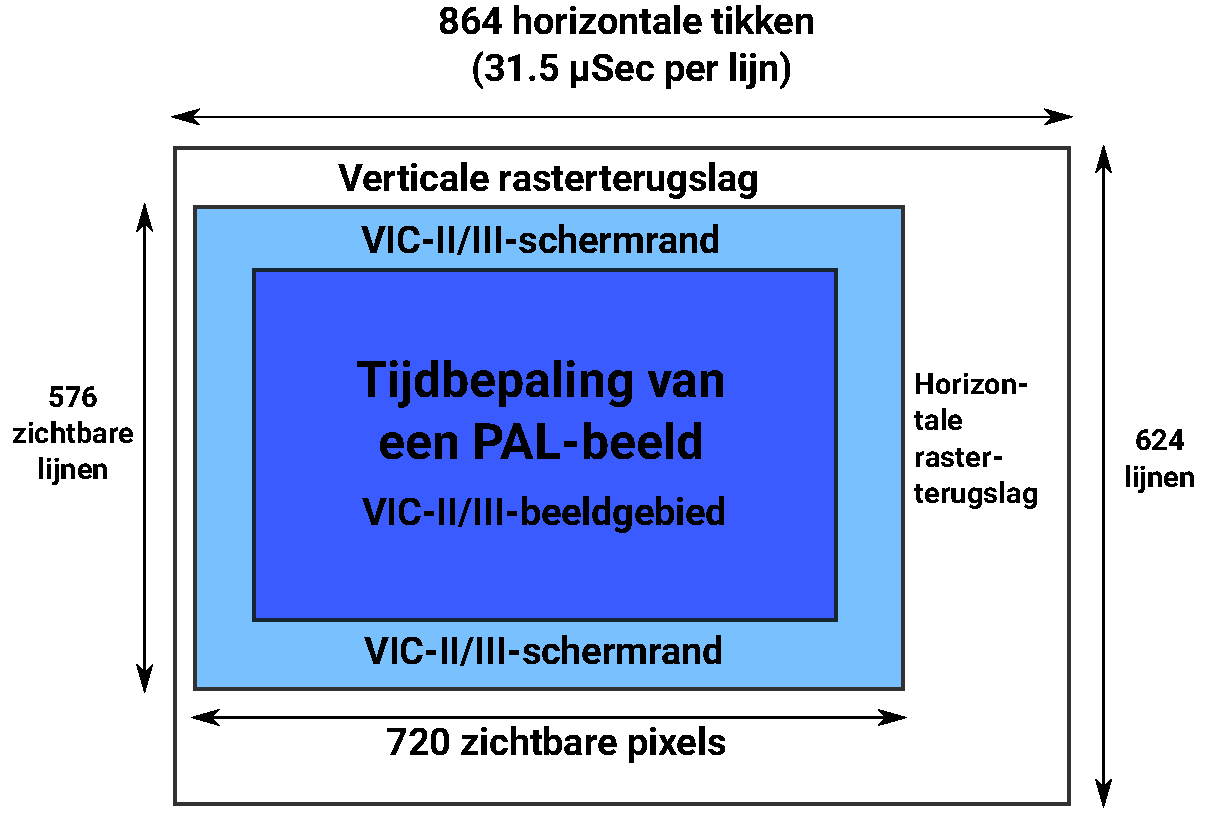
\includegraphics[width=\linewidth]{dutch/images/illustrations/VIC-IV-PAL-Frame.pdf}

Het NTSC-frame bestaat uit 526 fysieke rasterlijnen met elk 858 pixelklokken. De pixelklok is 27 MHz, oftewel 1/3 van de VIC-IV-pixelklok. Het zichtbare frame is 720$\times$480 pixels, waarvan het geheel in de VIC-IV-modus kan worden gebruikt. In de VIC-II- en VIC-III-modi verkleint het randgebied de bruikbare grootte tot 640$\times$400 pixels. In de VIC-II-modus en VIC-III 200H-modi wordt de weergave dubbelgescand, waarbij twee fysieke rasterlijnen van 32 microseconden overeenkomen met één VIC-II-stijl rasterlijn van 64 microseconden. Elk frame bestaat dus uit 263 VIC-II-rasterlijnen van elk 64 microseconden, overeenkomstig de meest voorkomende NTSC-videotiming van de C64.

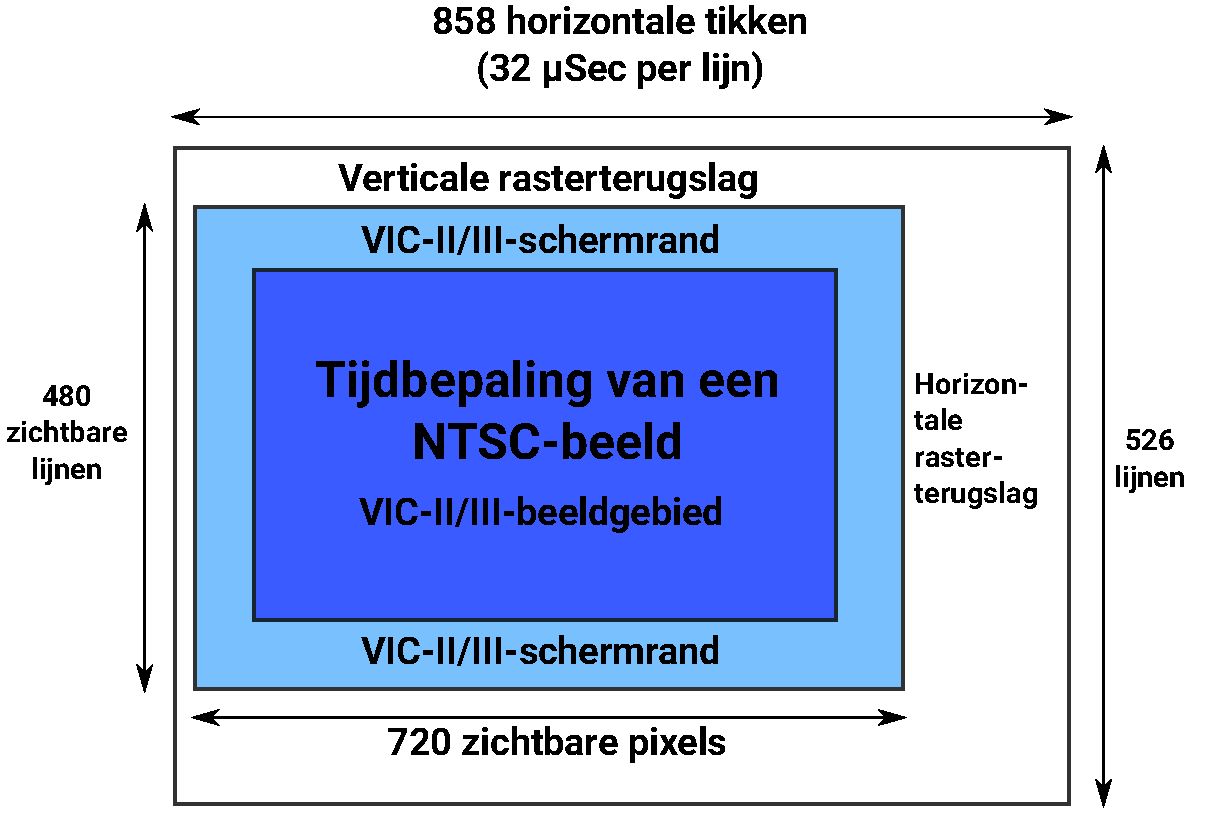
\includegraphics[width=\linewidth]{dutch/images/illustrations/VIC-IV-NTSC-Frame.pdf}

Omdat niet alle VGA-beeldschermen deze HDTV-videomodi ondersteunen, is er een compatibiliteitsmodus beschikbaar die een VGA-stijl modus van 640$\times$480 biedt. Omdat de pixelklok van de MEGA65 vaststaat op 27 MHz, werkt deze modus op 63 Hz. Dit zou op de overgrote meerderheid van VGA-beeldschermen moeten werken. Er zullen geen problemen optreden met de PAL/NTSC-modi bij gebruik van de digitale video-uitgang van de MEGA65 op de overgrote meerderheid van IMDH\texttrademark-compatibele beeldschermen en televisies.

Om te bepalen of de MEGA65 in PAL- of NTSC-modus werkt, kunt u het Freezer-menu openen, dat de huidige videomodus weergeeft, of vanuit een programma het PALNTSC-signaal controleren (bit 7 van \$D06F, decimaal 53359). Als deze bit gezet is, werkt het systeem in NTSC-modus; als deze gewist is, in PAL-modus. Deze bit kan worden gewijzigd om tussen de modi te schakelen, bijv.:

\begin{screencode}
10 REM C65+MEGA65-I/O INSCHAKELEN
20 IF PEEK($D018)<32 THEN POKE $D02F,ASC("G"):POKE $D02F,ASC("S")
30 REM NTSC-bit controleren
40 NTSC=PEEK($D06F) AND 128
50 REM STATUS WEERGEVEN EN OM OMSCHAKELING VRAGEN
60 PRINT"MEGA65 IS IN ";:IF NTSC THEN PRINT"NTSC MODE":ELSE PRINT"PAL MODE"
70 INPUT"SWITCH MODES (Y/N)? ",A$
80 REM NTSC-BIT OMSCHAKELEN
90 IF A$="Y" THEN POKE $D06F,PEEK($D06F) XOR 128:ELSE END
100 REM NIEUWE STATUS WEERGEVEN
110 NTSC=PEEK($D06F) AND 128
120 PRINT"MEGA65 IS IN ";:IF NTSC THEN PRINT"NTSC MODE":ELSE PRINT"PAL MODE"
\end{screencode}

\subsubsection{Fysieke en logische rasters}

Fysieke rasterlijnen per frame verwijzen naar het aantal daadwerkelijke rasterlijnen in de PAL- of NTSC-EDTV-videomodi die door de MEGA65 worden gebruikt. Logische rasterlijnen verwijzen naar het aantal VIC-II-stijl rasterlijnen per frame. Elke logische rasterlijn bestaat uit twee fysieke rasterlijnen per regel, aangezien EDTV-modi dubbelgescande modi zijn vergeleken met de oorspronkelijke PAL- en NTSC-SDTV-modi van de C64. De frame-parameters van de VIC-IV voor PAL en NTSC zijn als volgt:

\setlength{\tabcolsep}{3pt}
\begin{longtable}{|L{2cm}|L{2.5cm}|L{2.5cm}|L{2.5cm}|}
\hline
{\bf{Standaard}} & {\bf{Cycli per rasterlijn}} & {\bf{Fysieke rasterlijnen per frame}} & {\bf{Logische rasterlijnen per frame}}  \\
\hline
\endfirsthead
\multicolumn{3}{l@{}}{\ldots vervolg}\\
\hline
{\bf{Standaard}} & {\bf{Cycli per rasterlijn}} & {\bf{Fysieke rasterlijnen per frame}} & {\bf{Logische rasterlijnen per frame}}  \\
\hline
\endhead
\multicolumn{3}{l@{}}{vervolg \ldots}\\
\endfoot
\hline
\endlastfoot
	\small PAL & 63 & 626 & 312  \\	\small NTSC & 65 & 526 & 263  \\
\end{longtable}

Het resultaat is dat de frames op de VIC-IV exact hetzelfde aantal $\sim$1 MHz-CPU-cycli bevatten als op de VIC-II.

\subsubsection{Bad lines}

De VIC-IV kent van nature geen ``bad lines'', omdat de VIC-IV eigen geheugenbussen heeft naar het hoofdgeheugen en het kleurengeheugen (colour RAM) van de MEGA65. Hierdoor kunnen zowel de processor als de VIC-IV tegelijkertijd toegang krijgen tot het geheugen, in tegenstelling tot de C64 of C65, waarbij de toegang wordt afgewisseld.

Om de compatibiliteit te verbeteren, geeft de VIC-IV echter aan wanneer een ``bad line'' zou hebben plaatsgevonden op de VIC-II. De 45GS02-processor van de MEGA65 aanvaardt deze bad-line-signalen en onderbreekt de CPU gedurende 40 klokcycli, tenzij de processor op volle snelheid draait, in welk geval deze worden genegeerd. Dit verbetert de timingcompatibiliteit met de VIC-II aanzienlijk. De timing is echter niet exact, omdat de huidige revisie van de 45GS02 precies 40 cycli onderbreekt in plaats van 40--43 cycli, afhankelijk van de instructie die op dat moment wordt uitgevoerd. Daarnaast onderbreken de VIC-IV en 45GS02 momenteel niet voor sprite-ophaaloperaties.


De bad-line-emulatie wordt beheerd door bit 0 van \$D710: het zetten van deze bit schakelt bad-line-emulatie in, en het wissen ervan voorkomt dat een bad line tijd van de processor steelt.


\section{Geheugeninterface}

De VIC-IV ondersteunt tot 16 MB direct toegankelijk RAM voor videogegevens, maar momenteel bieden alle bestaande modellen slechts 384 KB adresseerbaar RAM. In MEGA65-systemen wordt het tweede blok van 128 KB RAM (in het geheugengebied van 128 KB tot 256 KB) doorgaans gebruikt om een C65-compatibele ROM op te slaan, waardoor 256 KB RAM voor de gebruiker beschikbaar blijft. Indien de software zo is geschreven dat het gebruik van C65-ROM-routines niet nodig is, kan de volledige 384 KB RAM door het programma worden gebruikt.

Alle MEGA65-modellen ondersteunen momenteel 32 KB kleurengeheugen (colour RAM), maar er zijn plannen om het nieuwste R3-bord 64 KB kleurengeheugen (of mogelijk zelfs 128 KB) te laten ondersteunen.

De VIC-IV ondersteunt alle methoden van de oudere VIC-II en VIC-III voor de toegang tot dit geheugen, waaronder het gebruik van 16KB-banken door de VIC-II en de Display Address Translator (DAT) van de VIC-III. Dit extra geheugen kan voor teken- en bitmapweergaven worden gebruikt, evenals voor sprites. De bitplanemodi van de VIC-III blijven echter beperkt tot het gebruik van slechts de eerste 128KB van het geheugen, omdat de VIC-IV de bitplanemodus niet uitbreidt.

\subsection{Schermgeheugen lokaliseren en verplaatsen}

De VIC kan worden geconfigureerd om het tekstschermgeheugen overal in de eerste 384KB te zoeken. Uw programma kan bepalen waar het schermgeheugen komt te staan en het startadres in de hardware-registers instellen. Dit adres wordt opgeslagen in de SCRNPTR-registers (\$D060 -- \$D063, 53344 -- 53347 decimaal). Om het schermgeheugen bijvoorbeeld op adres 12345 in te stellen:

\begin{screencode}
REM C65+MEGA65-I/O INSCHAKELEN
IF PEEK($D018)<32 THEN POKE $D02F,ASC("G"):POKE $D02F,ASC("S")

WPOKE $D060,$2345:POKE $D062,$1
\end{screencode}

Om een bestaand scherm te gebruiken dat door de KERNAL is ingesteld (het scherm dat de gebruiker bij het opstarten ziet), kunt u het startadres uit deze registers lezen. Houd er rekening mee dat de KERNAL in sommige omstandigheden de locatie van het schermgeheugen wijzigt. De beste praktijk is daarom dit adres binnen het programma uit de registers te lezen en de locatie ervan niet te veronderstellen.

\begin{screencode}
10 SC=WPEEK($D060)+(PEEK($D062)*65536)
20 POKE SC,1 : REM SCHRIJFT EEN "A" NAAR DE LINKERBOVENHOEK
\end{screencode}

\subsection{Tekengeneratorgegevens verplaatsen}

De locatie van de tekengeneratorgegevens kan eveneens met precisie op byteniveau worden ingesteld via de CHARPTR-registers op \$D068 -- \$D06A (53352 -- 53354 decimaal). Zoals gebruikelijk bevat het eerste van deze registers de minst significante byte en het laatste de meest significante byte. De drie bytes maken plaatsing van tekengeneratorgegevens overal in de eerste 16MB van het geheugen mogelijk. Voor systemen met minder dan 16MB geheugen waartoe de VIC-IV toegang heeft, dienen de bovenste adresbits op nul te staan.

Om bijvoorbeeld aan te geven dat de tekengeneratorgegevens vanaf \$41200 (266752 decimaal) moeten worden gelezen, kan het volgende worden gebruikt. Houd er rekening mee dat het commando WPOKE kan worden gebruikt om twee bytes als een woord naar een geheugen- of I/O-locatie te schrijven. Wij gebruiken daarom WPOKE om \$00 naar \$D068 en \$12 naar \$D069 te schrijven, en een extra POKE om de hoge byte \$A naar \$D06A te schrijven door het adres door 65536 te delen:

\begin{screencode}
REM C65+MEGA65-I/O INSCHAKELEN
IF PEEK($D018)<32 THEN POKE $D02F,ASC("G"):POKE $D02F,ASC("S")
REM HEX $41200 IS MAKKELIJK VERDEELD IN ZIJN 3 BYTES $00, $12, $4
REM WPOKE ZET DE ONDERSTE TWEE BYTES IN EEN COMMANDO EN
REM DE VOLGENDE POKE ZET DE BOVENSTE BYTE
A=$41200
WPOKE $D068,A
POKE $D06A,A/65536
\end{screencode}

\subsection{Het kleuren-/attribuutgeheugen verplaatsen}

Het gebruikte deel van het kleurengeheugen kan op vergelijkbare wijze worden ingesteld met de COLPTR-registers (\$D064 -- \$D065, 53348 -- 53349 decimaal). De waarde is namelijk een verschuiving vanaf het begin van het kleuren-/attribuutgeheugen. Dit komt omdat het kleuren-/attribuutgeheugen van de MEGA65, net als op de C64, een afzonderlijk geheugenonderdeel is met een eigen verbinding met de VIC-IV. Standaard zijn de COLPTR's op nul ingesteld, wat het gedrag van de VIC-II/III nabootst. Om de weergave het kleuren-/attribuutgeheugen vanaf verschuiving \$4000 te laten gebruiken, kan men bijvoorbeeld iets als het volgende gebruiken:

\begin{screencode}
REM C65+MEGA65-I/O INSCHAKELEN
IF PEEK($D018)<32 THEN POKE $D02F,ASC("G"):POKE $D02F,ASC("S")
REM STEL COLPTR IN OP $4000, VERDEELD IN $00-LSB en $40-MSB
POKE $D064,$00
POKE $D065,$40
\end{screencode}

\subsection{Spritepointers en sprite-afbeeldingen verplaatsen}

De locatie van de spritepointers kan eveneens worden verplaatst, en sprites kunnen hun gegevens overal in de eerste 4MB van het geheugen laten hebben. Dit wordt bereikt door eerst de locatie van de spritepointers in te stellen via de SPRPTRADR-registers (\$D06C -- \$D06E, 53356 -- 53358 decimaal; houd er echter rekening mee dat alleen de onderste 7 bits van \$D06E worden gebruikt, omdat de hoogste bit voor het SPRPTR16-signaal wordt gebruikt). Hierdoor kan de lijst van acht spritepointers van het einde van het schermgeheugen naar een willekeurige locatie in de eerste 8MB van het geheugen worden verplaatst. SPRPTRADR moet op een 16-byte-grens (een veelvoud van 16) zijn uitgelijnd.

Om sprites zelf overal in de eerste 4MB van het geheugen te kunnen plaatsen, moet de SPRPTR16-bit in \$D06E worden gezet. In deze modus worden twee bytes gebruikt om de locatie van elke sprite aan te geven, in plaats van één byte. De lijst van spritepointers is daardoor 16 bytes lang, in plaats van 8 bytes zoals op de VIC-II/III. Wanneer SPRPTR16 is ingeschakeld, moet de locatie van de spritepointers altijd expliciet via de SPRPTRADR-registers worden ingesteld.

Om de spritepointers bijvoorbeeld op locatie 800 -- 815 te plaatsen, kunt u min of meer de volgende code gebruiken. Houd er rekening mee dat enige kunstgrepen nodig zijn om de SPRPTR16-bit ongewijzigd te laten, en ook om de AND-binaire operator, die niet met waarden groter dan 65535 werkt, te omzeilen:

\begin{screencode}
REM C65+MEGA65-I/O INSCHAKELEN
IF PEEK($D018)<32 THEN POKE $D02F,ASC("G"):POKE $D02F,ASC("S")
POKE $D06C,(800-INT(800/65536)*65536) AND 255
POKE $D06D,INT(800/256) AND 255
POKE $D06E,(PEEK($D06E) AND 128)+INT(800/65536)
\end{screencode}

De locatie van elke sprite-afbeelding blijft een veelvoud van 64 bytes, waardoor er op elk moment tot 65,536 unieke sprite-afbeeldingen kunnen worden gebruikt, indien het systeem over voldoende geheugen beschikt (4MB of meer). In deze modus wordt de 16KB-banking van de VIC-II genegeerd, en is de locatie van de spritegegevens eenvoudigweg 64 $\times$ de pointerwaarde. Om de gegevens voor een sprite op \$C000 (49152 decimaal) te hebben, zou dit bijvoorbeeld sprite-locatie 768 zijn, omdat 49152 gedeeld door 64 = 768. Vervolgens moeten wij 768 in hoge en lage bytes splitsen om de twee pointerbytes in te stellen: 768 = 256$\times$3, met rest 0. Dit zou dus vereisen dat de twee spritepointerbytes 0 (lage byte, die als eerste komt) en 3 (hoge byte) zijn. Indien de spritepointers zich op \$7F8 (2040 decimaal) bevonden, zou het instellen van de eerste sprite op sprite-afbeelding 768 kunnen worden gedaan met zoiets als:

\begin{screencode}
POKE 2040,768-256*INT(768/256)
POKE 2041,INT(768/256)
\end{screencode}

\section{Hete registers}
\index{Hete registers}

Sommige VIC-IV-registers ondersteunen functies die vergelijkbaar zijn met die van de VIC-II en VIC-III, maar met uitgebreide mogelijkheden. Voor achterwaartse compatibiliteit zorgt het schrijven naar specifieke VIC-II- en VIC-III-registers er ook voor dat de bijbehorende VIC-IV-registers worden gereset met consistente waarden. Dit gedrag kan worden geconfigureerd met de HOTREG-vlag in bit 7 van \$D05D.

De onderste vier bits van register \$D018 (\textbf{CB}) stellen bijvoorbeeld het tekensetadres van de VIC-II in, als een veelvoud van 1 KiB. De VIC-IV kan de tekenset op elk 24-bits adres plaatsen met behulp van \$D06A (\textbf{CHARPTRBNK}), \$D068 (\textbf{CHARPTRLSB}) en \$D069 (\textbf{CHARPTRMSB}). Indien u CB instelt, worden de VIC-IV-registers ook bijgewerkt om hiermee overeen te komen.

De volledige reeks ``hete'' VIC-II-registers die van invloed zijn op de VIC-IV-registers omvat:

\begin{itemize}
\item \$D011 (53265): RB8, ECM, BMM, BLNK, RSEL, YSCL\item \$D016 (53270): RST, MCM, CSEL, XSCL\item \$D018 (53272): VS, CB\item \$D031 (53297): VIC-III-modi: H640, FAST, ATTR, BPM, V400, H1280, MONO, INT\item De VIC-II-bankbits van \$DD00 (56576) (CIA 2 PORTA)
\end{itemize}

Telkens wanneer een van die registers wordt gewijzigd, zelfs door de bestaande waarde er weer in terug te schrijven, worden alle bijbehorende VIC-IV-registers bijgewerkt op basis van de VIC-II-registerwaarden, zelfs die welke geen verband houden met het register waarnaar is geschreven. Dit omvat de FAST-vlag, welke zich op een byte-locatie van een heet register (\$D031) bevindt, maar geen verband houdt met de videoparameters en geen bijbehorend VIC-IV-register heeft.

De registers die tijdens dit proces worden gewijzigd, staan hieronder vermeld. Houd er rekening mee dat sommige van deze registers intern zijn aan de VIC-IV en niet rechtstreeks door de gebruiker kunnen worden opgevraagd of gewijzigd. Waar dit het geval is, worden er geen adressen voor de registers vermeld.

\begin{itemize}
\item {\bf X-positie van de linkerrandgrens.}  Dit interne register wordt bijgewerkt om de linkerrand in te stellen op de breedte die in de ``Single Side Border Width''-registers is aangegeven (\$D05C bevat de LSB, en bits 0 -- 5 van \$D05D bevatten de MSB van de breedte van de zijrand.  Houd er rekening mee dat de breedte van de zijrand is gebaseerd op de afmetingen van het videoframe op laag niveau, niet op de weergavegrootte van het scherm van de videomodus. Wanneer het 38/40-kolommenveld van \$D016 op 38 kolommen is ingesteld, verschijnt de linkerrandgrens 14 pixels rechts van zijn normale positie.\item {\bf X-positie van de rechterrandgrens.} Dit is hetzelfde als de linkerrandgrens, maar dan voor de rechterrand van het scherm. Houd er rekening mee dat wanneer de 38/40-kolommenvlag op 38 kolommen is ingesteld, de rechterrandgrens 17 pixels naar links van zijn normale positie wordt verplaatst.\item {\bf Y-positie van de bovenste randgrens (\$D048 LSB, bits 0 -- 3 van \$D049 MSB).} Dit interne register wordt ingesteld op de normale bovenste positie van het scherm, minus de waarde van het RASLINE0-veld in bits 0 -- 5 van \$D06F.  Wanneer het 24/25-rijenveld van \$D011 op 24 rijen is ingesteld, wordt de bovenste randgrens met 8 rasterlijnen verlaagd.\item {\bf Y-positie van de onderste randgrens (\$D04A LSB, bits 0 -- 3 van \$D04B MSB).} Dit interne register wordt ingesteld op de normale bovenste positie van het scherm, plus 400 rasterlijnen, om het normale 400px hoge primaire weergavegebied binnen de randen te creëren. Wanneer het 24/25-rijenveld van \$D011 op 24 rijen is ingesteld, wordt de bovenste randgrens met 8 rasterlijnen verhoogd.\item {\bf Verticale schaal van de tekengenerator (\$D05B).} Dit register wordt ingesteld op 0 voor de V200- of 1 voor de V400-modus, zodat elke pixelrij in een teken respectievelijk 1 of 2 pixels hoog wordt, volgens de V400-vlag.\item {\bf Aantal weer te geven tekenrijen (\$D07B).} Dit register wordt ingesteld op 25-1 = 24 of 50-1 = 49 om respectievelijk 25 of 50 tekstrijen weer te geven.  Houd er rekening mee dat wanneer \$D011 wordt gebruikt om de verticale randen naar binnen te brengen om het aantal zichtbare tekenrijen te verminderen, de VIC-IV nog steeds alle 25 of 50 rijen tekent.\item {\bf X-positie waar de tekenweergave begint (\$D04C LSB, bits 0 -- 3 van \$D04D MSB).}  Dit register wordt ingesteld op een positie ten opzichte van de rand van het 40-kolommen brede tekstscherm, plus 2$\times$ de positie van de vloeiende verschuiving die in \$D016 is aangegeven.\item {\bf Y-positie waar de tekenweergave begint (\$D04E LSB, bits 0 -- 3 van \$D04F MSB).}  Dit register wordt ingesteld op de bovenrand van de verticale rand, minus het VIC-II First Raster-aanpassingsregister (bits 0 -- 5 van \$D06F), plus eventuele verschuiving als gevolg van de verticale bits voor vloeiende verschuiving in \$D011.\item {\bf Virtuele rijbreedte (\$D058 LSB, \$D059 MSB), d.w.z. het aantal bytes scherm- en kleurengeheugen waarmee de VIC-IV vooruitgaat bij het weergeven van elke opeenvolgende tekenrij.} Dit register wordt ingesteld op 40 als de H640-vlag is gewist, of op 80 als de H640-vlag is gezet, waardoor de voortgang overeenkomt met het aantal weer te geven tekens.\item {\bf Breedte van de weergaverij (\$D05E LSB, bits 4 -- 5 van \$D063 MSB).} Dit register wordt ingesteld op 40 als de H640-vlag is gewist, of op 80 als de H640-vlag is gezet.\item {\bf Basisadres van het schermgeheugen (\$D060 -- \$D062, dat een 24-bits adres voorstelt).}  Dit adres wordt gereset naar het adres zoals berekend aan de hand van \$D018 en \$DD00, zoals op de C64.\item {\bf Spritepointer-adres van de VIC-II (\$D06C -- \$D06E, dat een 24-bits adres voorstelt).} Dit register wordt gereset naar de normale locatie aan het einde van het schermgeheugen van de huidige modus.  Indien de H640-vlag is gezet, gebeurt dit aan het einde van het 2KB-gebied van het schermgeheugen, of indien de H640-vlag niet is gezet, wijst het naar het einde van het 1KB-gebied van het schermgeheugen, zoals op een C64.\item {\bf Basisadres van de tekenset (\$D068 -- \$D06A, dat een 24-bits adres voorstelt).}  Houd er rekening mee dat de hete registerfunctie alleen de onderste 16 bits van het tekensetadres instelt. Dat wil zeggen dat \$D06A niet wordt gewist. Dit is bewust gedrag, waardoor het gemakkelijker wordt om in bestaande VIC-II-georiënteerde software de tekenset te vervangen door een andere tekenset in een andere geheugenbank.\item {\bf Basisadres van het kleurengeheugen (\$D064 LSB, \$D065 MSB).} Deze registers worden naar nul gereset, waardoor de VIC-IV verwacht dat het kleurengeheugen voor het scherm zich in het eerste deel van het kleurengeheugen bevindt, om compatibel te zijn met de VIC-II en VIC-III.
\end{itemize}

Dit gedrag van de VIC-II-registers is vooral bedoeld voor software uit het verleden die geen weet heeft van (en daarom nooit naar) VIC-IV-registers schrijft. De hete-registerpropagatie kan worden uitgeschakeld door het HOTREG- (``hete register'') signaal te wissen: bit 7 van \$D05D (53341). Indien u de HOTREG-vlag wist, moet u de VIC-IV-registers rechtstreeks bijwerken wanneer u de parameters van de videomodus wilt wijzigen.

Indien u een wijziging in een heet register aanbrengt terwijl HOTREG is uitgeschakeld en HOTREG vervolgens weer inschakelt, worden alle hete registers onmiddellijk bijgewerkt. Er zijn zeldzame gevallen waarin u een wijziging in een heet register wilt aanbrengen zonder de VIC-IV-registers bij te werken, maar de hete registers na de wijziging toch ingeschakeld wilt hebben. Om dit te doen, kunt u de openstaande bijwerking annuleren door vlak voordat u de hete registers weer inschakelt opnieuw een 0 naar HOTREG te schrijven. De volledige procedure is:

\begin{enumerate}
\item Schrijf 0 naar HOTREG om hete registers uit te schakelen.\item Werk het VIC-II-register bij dat u wilt wijzigen.\item Schrijf 0 naar HOTREG om de openstaande bijwerking te annuleren.\item Schrijf 1 naar HOTREG om hete registers weer in te schakelen.
\end{enumerate}

In assembleertaal:

\begin{screencode}
lda #%10000000
trb $d05d        ; hete registers uitschakelen

lda #%01000000
tsb $d031        ; een VIC-II/III-register bijwerken

lda #%10000000
trb $d05d        ; openstaande bijwerking wissen
tsb $d05d        ; hete registers weer inschakelen
\end{screencode}


\section{Nieuwe modi}

\subsection{Waarom de nieuwe VIC-IV-modi teken- en bitmapmodi zijn en geen bitplanemodi}

De nieuwe videomodi van de VIC-IV zijn afgeleid van de teken- en bitmapmodi van de VIC-II, in plaats van de bitplanemodi van de VIC-III. Deze keuze was gebaseerd op diverse praktische aspecten van het programmeren van een geheugenbeperkte 8-bit thuiscomputer:

\begin{enumerate}
\item Bitplanes vereisen dat dezelfde hoeveelheid geheugen aan elk gebied op het scherm wordt toegewezen, ongeacht of het lege ruimte of complexe afbeeldingen weergeeft. Met bitplanes is het niet mogelijk om inhoud uit een afbeelding opnieuw te gebruiken in een ander deel van die afbeelding. De meeste C64-spellen maken echter gebruik van sterk repetitieve schermen, waarbij veelgebruikte elementen op diverse plaatsen op het scherm voorkomen, waarvan Boulder Dash en Super Giana Sisters goede voorbeelden zijn.

\item Bitplanes maken het ook moeilijk om een beeldscherm bij te werken, omdat elke pixel uniek is: er is geen mogelijkheid om een wijziging, bijvoorbeeld in de animatie van een schermelement, door te voeren op alle plaatsen tegelijk. De diamantanimaties in Boulder Dash zijn een goed voorbeeld van dit probleem. Het moeten wijzigen van meerdere afzonderlijke bytes in elke bitplane vormt een verhoogde rekenkundige belasting, hetgeen de reden was dat er voor de Amiga AAA-chipset werd gevraagd zogenaamde ``chunky''-modi op te nemen, in plaats van uitsluitend op bitplanes gebaseerde modi. Hoewel de Display Address Translator (DAT) en DMAgic van de C65 enige verlichting bieden voor dit probleem, is die verlichting slechts gedeeltelijk.

\item Scrollen met behulp van de bitplanes van de C65 vereist het kopiëren van de gehele bitplane, omdat de hardwareondersteuning voor vloeiend scrollen zich niet uitstrekt tot het op fijne wijze wijzigen van het bronadres van de bitplane. Zelfs met gebruikmaking van de DMAgic vereist het scrollen van een 320$\times$200 256-kleurenscherm in het gunstigste geval 128.000 klokcycli (het lezen en schrijven van 320$\times$200 = 64.000 bytes). Op 3.5 MHz op de C65 zou dit ongeveer 36 milliseconden kosten, oftewel ongeveer 2 volledige videoframes. Voor vloeiend scrollen van een dergelijk scherm is daarom een dubbelgebufferde regeling nodig, die 128.000 van de 131.072 bytes geheugen zou verbruiken.

De bekende tekenmodi van de VIC-II worden daarentegen veelvuldig in spellen gebruikt, omdat ze met een geringe hoeveelheid schermgeheugen kunnen bepalen welk blok van 8$\times$8 pixels wordt weergegeven, wat zeer snel scrollen, minder geheugengebruik en effectieve hardwareversnelling van animatie van veelgebruikte elementen mogelijk maakt. De verbeteringen in de VIC-IV zijn dan ook vooral op de tekenmodus gericht. Omdat de bitmapmodus op de VIC-II feitelijk een speciaal geval van de tekenmodus is, met impliciete tekennummers, wordt deze op de VIC-IV als het ware gratis meegeleverd en zal alleen in het kader van een zeer klein aantal bitmapmodus-specifieke verbeteringen worden genoemd die triviaal te implementeren waren en waarvan het dus onverstandig leek ze niet te realiseren, voor het geval ze toch van pas komen.

\end{enumerate}

\subsection{Weergeven van meer dan 256 unieke tekens via ``Super-Uitgebreide Attribuutmodus''}

De belangrijkste innovatie is de toevoeging van de Super-Uitgebreide Attribuutmodus (SEAM). De VIC-II gebruikt al 12 bits per teken: elke cel van 8$\times$8 pixels wordt gedefinieerd door 12 bits gegevens: 8 bits schermgeheugengegevens, standaard van \$0400 -- \$07E7 (1024 -- 2023 decimaal), die aangeven welke tekens moeten worden weergegeven, en 4 bits kleurgegevens van het 1 KB nibble kleurengeheugen op \$D800 -- \$DBFF (55296 -- 56319 decimaal). De VIC-III van de C65 gebruikt 16 bits, omdat het kleurengeheugen nu 8 bits telt in plaats van 4, waarbij de extra 4 bits kleurengeheugen worden gebruikt om attributen te ondersteunen (knipperen, vet, onderstrepen en inverse weergave). Het wordt aanbevolen om de werking hiervan door te nemen voordat u verder leest. Een goede inleiding op de tekstmodus van de VIC-II is op veel plaatsen te vinden.
% For example, \ref{vicii-cheaper-by-the-dozen}. <- undefined
Super-Uitgebreide Attribuutmodus verdubbelt het aantal bits per teken van de 16 van de VIC-III tot 32: twee bytes schermgeheugen en twee bytes kleuren-/attribuutgeheugen.

Super-Uitgebreide Attribuutmodus wordt ingeschakeld door bit 0 in \$D054 (53332 decimaal) te zetten. Vergeet niet eerst de VIC-IV-modus in te schakelen om dit register toegankelijk te maken. Wanneer deze bit is gezet, worden twee bytes gebruikt voor zowel het schermgeheugen als het kleurengeheugen voor elk teken dat op het scherm wordt weergegeven. In vergelijking met de 12 bits informatie die de C64 per teken gebruikt en de 16 bits van de VIC-III, heeft de VIC-IV 32 bits informatie. Hoe deze 32 bits worden gebruikt, varieert enigszins per modus, zoals beschreven in de volgende tabellen, inclusief of de GOTOX-bit is gezet.

Let er ook op dat het tegelijkertijd inschakelen van de BOLD- en REVERSE-attributen op de MEGA65 een alternatief palet selecteert, waardoor feitelijk 512 kleuren op het scherm mogelijk zijn, maar elk 8$\times$8-teken slechts kleuren uit één palet van 256 kleuren kan gebruiken.

De twee tabellen die volgen beschrijven de bitvelden die voor dit teken beschikbaar zijn, die variëren afhankelijk van of de \textbf{GOTOX\_flag} is gezet of gewist:

\begin{itemize}
  \item \textbf{GOTOX\_flag = 0} creëert een \underline{zichtbaar teken} (\textcolor{blue}{blauwe} bitvelden) met attributen die \underline{dit teken} beïnvloeden.  \item \textbf{GOTOX\_flag = 1} creëert een \underline{onzichtbaar teken} (\textcolor{red}{rode} bitvelden) met attributen die \underline{volgende tekens} beïnvloeden.
\end{itemize}


% Force table to sit on a single page for more convenient reading.
% ensures that they are both visible on the same open page :)
% (\cleardoublepage does the opposite)
\clearpage
\ifodd\value{page}\hbox{}\newpage\fi
\subsubsection{Bitvelden indien GOTOX\_flag is gewist:}

\setlength{\tabcolsep}{3pt}
\begin{longtable}{|L{2.1cm}|L{9cm}|}
  \hhline{==}
  {\bf{Bit(s)}} & {\bf{Functie wanneer GOTOX\_flag is \underline{\textcolor{blue}{gewist}}}}  \\
  \hhline{==}
\endfirsthead
\multicolumn{2}{l@{}}{\ldots vervolg}\\
  \hhline{==}
  {\bf{Bit(s)}} & {\bf{Functie wanneer GOTOX\_flag is \underline{\textcolor{blue}{gewist}}}}  \\
  \hhline{==}
\endhead
\multicolumn{2}{l@{}}{vervolg \ldots}\\
\endfoot
\hline
\endlastfoot
  \hline
  \multicolumn{2}{|l|}{\small \textbf{Schermgeheugen-byte 0}} \\
  \hline
  \small \qquad Bits 7 - 0 & {\small \textbf{\textcolor{blue}{char\_number (lo)}}: (bits 7 -- 0) Laagste byte van tekennummer\newline  (hetzelfde als de VIC-II en VIC-III) }\\
  \hline
  \multicolumn{2}{|l|}{\small \textbf{Schermgeheugen-byte 1}} \\
  \hline
  \small \qquad Bits 7 -- 5 & {\small \textbf{\textcolor{blue}{rhs\_trim (lo)}}: (bits 2 -- 0) Pixels aan de rechterkant van het teken wegsnijden)}\\
  \hline
  \small \qquad Bits 4 - 0 & {\small \textbf{\textcolor{blue}{char\_number (hi)}}: (bits 12 -- 8) Bovenste 5 bits van tekennummer, waardoor 8.192 unieke tekens kunnen worden aangesproken }\\
  \hline
  \multicolumn{2}{|l|}{\small \textbf{Kleurengeheugen-byte 0}} \\
  \hline
  \small \qquad Bit 7 & {\small \textbf{\textcolor{blue}{vert\_flip}}: het teken verticaal spiegelen }\\
  \hline
  \small \qquad Bit 6 & {\small \textbf{\textcolor{blue}{horz\_flip}}: het teken horizontaal spiegelen }\\
  \hline
  \small \qquad Bit 5 & {\small \textbf{\textcolor{blue}{alpha\_mode}}: de alpha-blendmodus inschakelen. De pixelwaarden worden dan als alpha-waarden behandeld die tussen de voorgrondkleur en de achtergrondkleur mengen (hiervoor moet \$D054.7 - ALPHEN worden ingesteld) }\\
  \hline
  \small \qquad \textbf{Bit 4} & {\small \textbf{GOTOX\_flag} is \textbf{\underline{\textcolor{blue}{gewist}} (op 0 gesteld)} \linebreak Verschaft de \textcolor{blue}{blauwe} bitvelden die in deze tabel worden getoond. Dit zijn attributen die invloed hebben op \underline{dit teken}. }\\
  \hline
  \small \qquad Bit 3 & {\small \textbf{\textcolor{blue}{ncm\_flag}}:
\begin{itemize}
  \item 1 = \underline{NCM-teken}: gebruikt 4 bits per pixel en is 16 pixels breed (minus eventuele trim-bits aan de rechterkant)  \item 0 = \underline{FCM-teken}: gebruikt 8 bits per pixel en is 8 pixels breed (minus eventuele trim-bits aan de rechterkant)
\end{itemize} }\\
  \hline
  \small \qquad Bit 2 & {\small \textbf{\textcolor{blue}{rhs\_trim (hi)}}: (bit 3) pixels aan de rechterkant van het teken wegsnijden}\\
  \hline
\small \qquad Bits 1 -- 0 & {\small GERESERVEERD, op 0 gesteld }\\
  \hline
  \multicolumn{2}{|l|}{\small \textbf{Kleurengeheugen-byte 1}} \\
  \hline
  \multicolumn{2}{|l|}{\small \quad \underline{Indien de VIC-II-multicolourmodus is ingeschakeld}: (\$D016.4 - MCM)} \\
  \hline
  \small \qquad Bits 7 -- 4 & {\small \textbf{\textcolor{blue}{colour (hi)}}: bovenste 4 bits van de voorgrondkleur van het teken}\\
  \hline
  \multicolumn{2}{|l|}{\small \quad \underline{Indien de uitgebreide attributen van de VIC-III zijn ingeschakeld}: (\$D031.5 - ATTR)} \\
  \hline
  \small \qquad Bit 7 & {\small \textbf{\textcolor{blue}{underline}}: Hardwarematige onderstreping van het teken }\\
  \hline
  \small \qquad Bit 6 & {\small \textbf{\textcolor{blue}{bold}}: Vetattribuut van het teken (hardware) * }\\
  \hline
  \small \qquad Bit 5 & {\small \textbf{\textcolor{blue}{reverse}}: Omgekeerde weergave van het teken (hardware) * }\\
  \hline
  \small \qquad Bit 4 & {\small \textbf{\textcolor{blue}{blink}}: Knipperen van het teken (hardware)}\\
  \hline
  \multicolumn{2}{|l|}{\small \quad \underline{Het overgebleven bitveld is gemeenschappelijk}:} \\
  \hline
\small \qquad Bits 3 -- 0 & {\small \textbf{\textcolor{blue}{colour (lo)}}: onderste 4 bits van de voorgrondkleur van het teken }\\
\end{longtable}

% Force table to sit on a single page for more convenient reading.
\newpage
\subsubsection{Bitvelden indien GOTOX\_flag is ingesteld:}

\setlength{\tabcolsep}{3pt}
\begin{longtable}{|L{2.1cm}|L{9cm}|}
  \hhline{==}
  {\bf{Bit(s)}} & {\bf{Functie wanneer GOTOX\_flag is \underline{\textcolor{red}{ingesteld}}}}  \\
  \hhline{==}
\endfirsthead
\multicolumn{2}{l@{}}{\ldots vervolg}\\
  \hhline{==}
  {\bf{Bit(s)}} & {\bf{Functie wanneer GOTOX\_flag is \underline{\textcolor{red}{ingesteld}}}}  \\
  \hhline{==}
\endhead
\multicolumn{2}{l@{}}{vervolg \ldots}\\
\endfoot
\hline
\endlastfoot
  \hline
  \multicolumn{2}{|l|}{\small \textbf{Schermgeheugen-byte 0}} \\
  \hline
  \small \qquad Bits 7 - 0 & {\small \textbf{\textcolor{red}{gotox\_pos (lo)}}: (bits 7 -- 0) onderste 8 bits van de nieuwe X-positie waar \underline{volgende tekens} moeten beginnen met tekenen, ten opzichte van het begin van het tekenen van het teken.  Door dit op 0 te stellen wordt het volgende teken over het meest linkse teken heen getekend. }\\
  \hline
  \multicolumn{2}{|l|}{\small \textbf{Schermgeheugen-byte 1}} \\
  \hline
  \small \qquad Bits 7 - 5 & {\small \textbf{\textcolor{red}{fcm\_yoffs}}: Y-offset van FCM-tekengegevens: wanneer niet nul, worden FCM-tekengegevens opgehaald vanaf het tekenadres + 8 $\times$ de Y-waarde, wat equivalent is aan één pixellijn FCM-tekengegevens per Y. Door zorgvuldig plannen kan dit worden gebruikt om meerdere lagen RRB-inhoud soepel verticaal te scrollen.  }\\
  \hline
  \small \qquad Bit 4 & {\small \textbf{\textcolor{red}{fcm\_yoffs\_dir}}: wanneer ingesteld, wordt het \textbf{\textcolor{red}{fcm\_yoffs}}-veld in plaats daarvan in mindering gebracht. }\\
  \hline
\small \qquad Bits 3 - 2 & {\small GERESERVEERD, op 0 ingesteld }\\
  \hline
  \small \qquad Bits 1 - 0 & {\small \textbf{\textcolor{red}{gotox\_pos (hi)}}: (bits 9 -- 8) bovenste 2 bits van de nieuwe X-positie (het hoogste bit is het tekenbit van het tweecomplement) }\\
  \hline
  \multicolumn{2}{|l|}{\small \textbf{Kleurengeheugen-byte 0}} \\
  \hline
  \small \qquad Bit 7 & {\small \textbf{\textcolor{red}{transparent\_flag}}: wanneer ingesteld, worden achtergrond-/transparante pixels niet getekend voor \underline{volgende tekens}, waardoor lagen mogelijk zijn }\\
  \hline
  \small \qquad Bit 6 & {\small \textbf{\textcolor{red}{background\_flag}}: wanneer ingesteld, worden \underline{volgende tekens} als achtergrond gerenderd, waardoor sprites ervoor kunnen verschijnen, zelfs wanneer sprites op achtergrond zijn ingesteld. }\\
  \hline
\small \qquad Bit 5 & {\small GERESERVEERD, op 0 ingesteld }\\
  \hline
  \small \qquad \textbf{Bit 4} & {\small \textbf{GOTOX\_flag} is \textbf{\textcolor{red}{op 1 ingesteld}}. Biedt de in deze tabel getoonde \textcolor{red}{rode} bitvelden, dit zijn attributen die \underline{volgende tekens} beïnvloeden. Eén opvallend veld is \textbf{\textcolor{red}{gotox\_pos}}, dat later in de sectie Raster-Rewrite Buffer wordt besproken.)}\\
  \hline
  \small \qquad Bit 3 & {\small \textbf{\textcolor{red}{rowmask\_flag}}: wanneer ingesteld, beslist het \textbf{\textcolor{red}{rowmask}}-veld welke pixellijnen van \underline{volgende tekens} moeten worden gerenderd. Dit kan worden gebruikt om tekens verticaal te scrollen met RRB, door elk teken op twee rijen te tekenen: verschoven naar beneden op de bovenste rij, en verschoven omhoog op de onderste rij, en gemaskeerd zodat alleen de pixellijnen van het gescrollde teken worden weergegeven, en niet de gegevens van vóór/na de gegevens van dat teken.}\\
  \hline
  \small \qquad Bit 2 & {\small \textbf{\textcolor{red}{foreground\_flag}}: wanneer ingesteld, worden \underline{volgende tekens} als voorgrond getekend, ongeacht hun kleur, waardoor sprites erachter kunnen verschijnen. }\\
  \hline
\small \qquad Bits 1 - 0 & {\small GERESERVEERD, op 0 ingesteld }\\
  \hline
  \multicolumn{2}{|l|}{\small \textbf{Kleurengeheugen-byte 1}} \\
  \hline
  \small \qquad Bits 7 - 0 & {\small \textbf{\textcolor{red}{rowmask}}: maskerwaarden voor pixellijnen. Bits 7 -- 0 = Rijen 7 -- 0.\newline 1 = rij weergeven, 0 = rij verbergen }\\
\end{longtable}


We zien dat we nog steeds de onderste 8 bits van het tekennummer in de C64-stijl hebben in de eerste schermgeheugen-byte. De tweede byte van het schermgeheugen krijgt daarvoor vijf extra bits, waardoor er 2$^{13}$ = 8.192 verschillende tekens op één scherm kunnen worden gebruikt. Dat is meer dan voldoende voor unieke tekens die een 80$\times$50-scherm bestrijken (wat mogelijk is om te maken met de VIC-IV).  De resterende bits maken het bijsnijden van het teken mogelijk.  Hierdoor kunnen tekens met variabele breedte worden gebruikt, waarmee dingen gedaan kunnen worden die normaal niet mogelijk zouden zijn, zoals het gebruik van tekstmodus voor vrije horizontale plaatsing van tekens (of delen daarvan). Dit werd oorspronkelijk toegevoegd om hardwarematige ondersteuning voor proportionele breedte-lettertypen mogelijk te maken.

Voor het kleurengeheugen is de tweede byte (byte 1) gelijk aan die van de C65, oftewel de onderste helft biedt vier bits voor de voorgrondkleur, zoals op de C64, plus de optionele VIC-III uitgebreide attributen. Het C65-specificatiedocument beschrijft het gedrag wanneer meer dan één van deze tegelijk wordt gebruikt, waarvan de meeste logisch zijn, maar er zijn een paar combinaties die zich anders gedragen dan verwacht. Het combineren van vetgedrukt met knipperen zorgt er bijvoorbeeld voor dat het teken schakelt tussen de vetgedrukte en de normale modus. Vetgedrukte modus zelf wordt geïmplementeerd door effectief te fungeren als bit 4 van de voorgrondkleurwaarde, waardoor de kleur van andere paletposities wordt getekend dan normaal.

Indien u de VIC-III uitgebreide attributen niet nodig heeft, kunt u in plaats daarvan de bovenste vier bits van de tweede byte van het kleurengeheugen gebruiken om meer bits van de kleurindex te bevatten, waardoor een selectie uit het volledige bereik van 256 kleurinstellingen mogelijk is.  Deze modus wordt geactiveerd door de multicolourmodus van de VIC-II in te schakelen terwijl de volledige kleurmodus actief is.

De C65 / VIC-III-attributen en het gebruik van 256-kleuren 8-bit-waarden voor verschillende VIC-II-kleurregisters wordt ingeschakeld door bit 5 van \$D031 (53297 decimaal) in te stellen.  Het wordt sterk aanbevolen dit te doen bij het gebruik van de VIC-IV-modus, omdat anders bepaalde functies niet naar behoren werken. Merk op dat BOLD+REVERSE samen de betekenis heeft van het selecteren van een alternatief palet op de MEGA65, wat verschilt van de C65.

Dankzij Super-Uitgebreide Attribuutmodus zijn veel effecten mogelijk.  Een paar mogelijkheden worden in de volgende subsecties uitgelegd.

\subsection{Super-Uitgebreide Attribuutmodus gebruiken}

Super-Uitgebreide Attribuutmodus vereist twee keer zoveel schermgeheugen en kleurengeheugen als de VIC-II/III-tekstmodi. Dit komt doordat er twee bytes van elk nodig zijn om elk teken te definiëren, in plaats van één.  Het schermgeheugen kan op elke willekeurige locatie in het 384KB hoofdgeheugen worden geplaatst met behulp van de registers \$D060 -- \$D062 (53344 -- 53346 decimaal).  Het kleurengeheugen kan op elke willekeurige locatie in het 32KB kleurengeheugen worden geplaatst.  Alleen de eerste 1 of 2KB van het kleurengeheugen is zichtbaar op \$D800 -- \$DBFF of \$D800 -- \$DFFF (indien het {\em CRAM2K}-signaal is ingesteld in bit 0 van \$D030, 53296 decimaal).  Indien een scherm groter dan 40$\times$25 tekens wordt gebruikt, is het gebruik van de DMA-controller of een andere manier vereist om het volledige kleurengeheugen te benaderen.  We bespreken daarom eerst het gebruik van Super-Uitgebreide Attribuutmodus met een 40x25-tekenweergave.

De eerste stap is het inschakelen van Super-Uitgebreide Attribuutmodus door de {\em FCLRHI}- en {\em CHR16}-signalen te activeren, door bits 2 en 0 van \$D054 (53332 decimaal) in te stellen.  Aangezien dit een VIC-IV-register is, moet eerst de VIC-IV I/O-modus worden ingeschakeld.  De VIC-IV moet ook worden geconfigureerd naar 40-kolomsmodus, door het {\em H640}-signaal uit te schakelen door bit 7 van \$D031 (53297 decimaal) te wissen.  Dit komt doordat elk tekenpaar samen één teken op het scherm vormt, waarbij één teken twee schermgeheugenbytes vereist, waardoor er 80 schermgeheugenbytes nodig zijn om 40 tekens weer te geven.  Eveneens zijn er 80 kleurengeheugenbytes nodig.

Om dit visueel te begrijpen, is het nuttig eerst de normale C64-schermgeheugenindeling te bekijken:

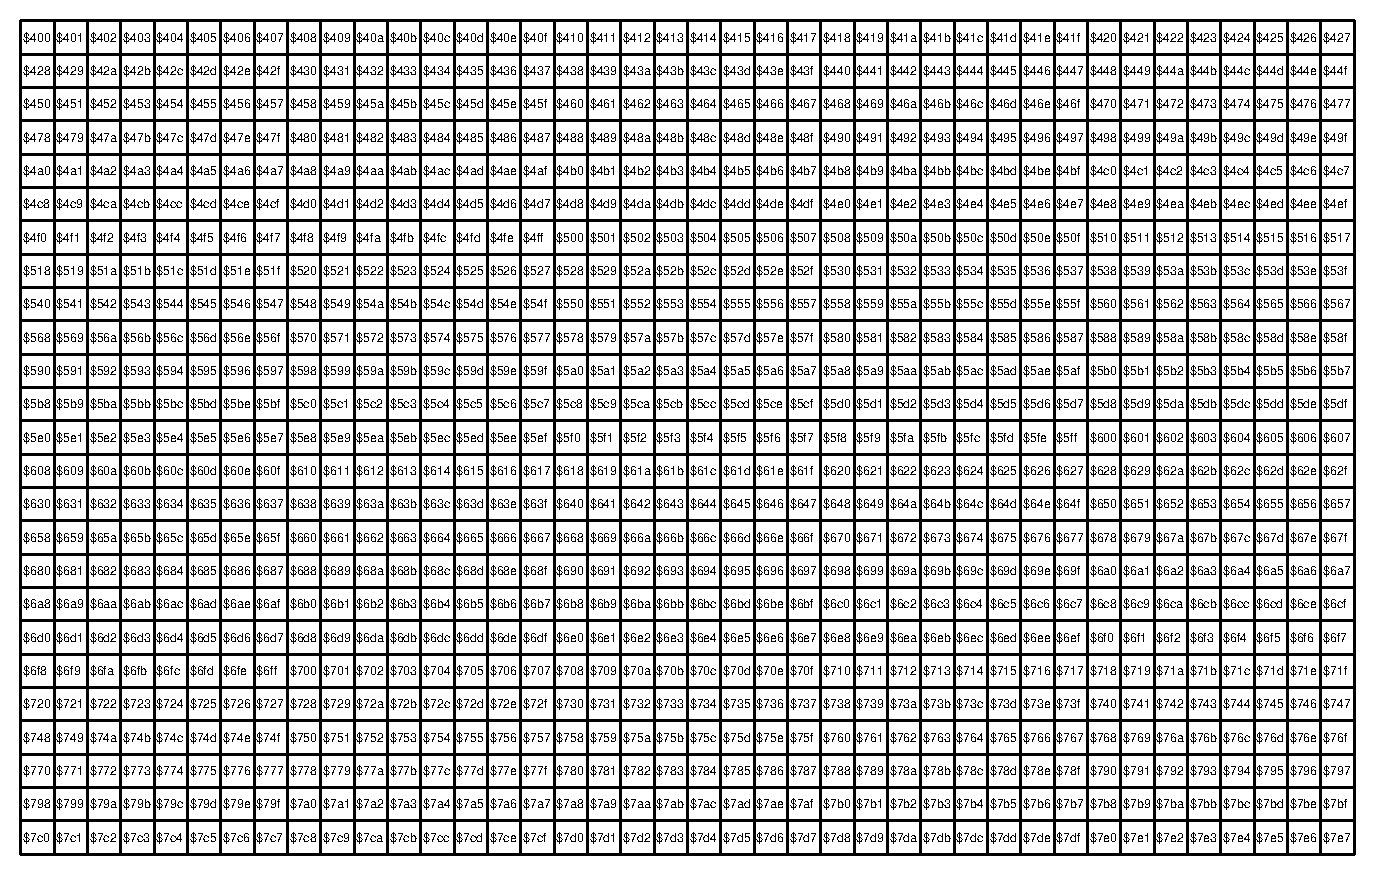
\includegraphics[width=\linewidth]{images/illustrations/screen-40x25-addresses.pdf}

Dat wil zeggen: elk tekencel gebruikt één byte van het schermgeheugen en de adressen nemen geleidelijk toe, zowel binnen regels als tussen regels. Super-Uitgebreide Attribuutmodus vereist twee bytes per tekencel. Indien u \$D054 bijvoorbeeld op \$05 instelt, krijgt u schermadressen als volgt:

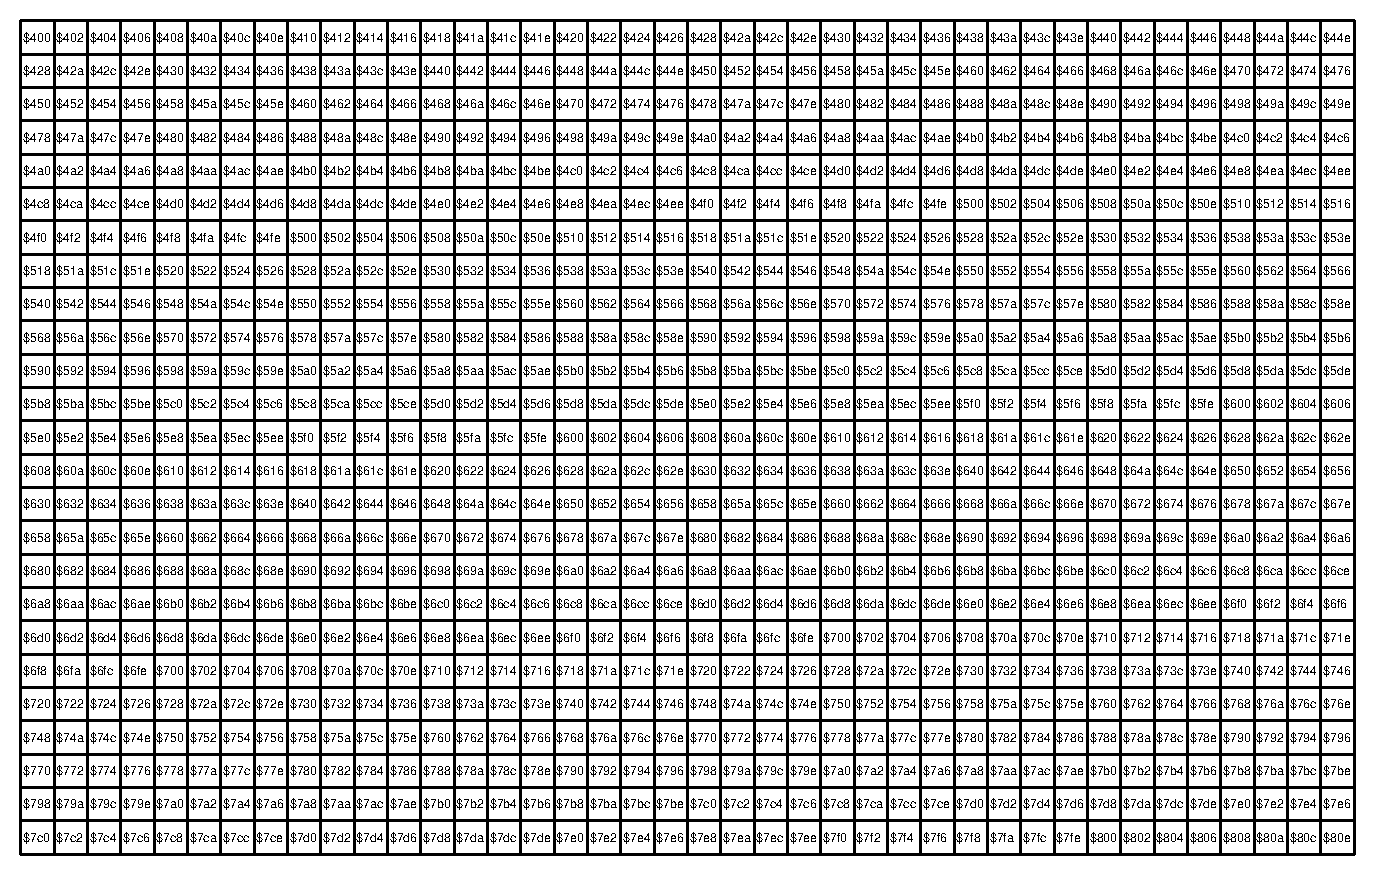
\includegraphics[width=\linewidth]{images/illustrations/screen-40x25-addresses16.pdf}

Er zijn twee zaken op te merken in de bovenstaande tabel: ten eerste vordert het adres met twee bytes per tekencel, omdat twee bytes nodig zijn om elk teken te definiëren. Ten tweede neemt het startadres van elke schermregel nog steeds slechts met 40 (\$28 in hexadecimaal) toe. Dit is niet wat we eigenlijk willen, want het betekent dat de eerste helft van de vorige regel opnieuw wordt weergegeven op elke huidige regel. Dit wordt opgelost door het aantal bytes dat per schermregel wordt overgeslagen in te stellen via \$D058 (LSB) en \$D059 (MSB). In dit geval willen we het aantal over te slaan bytes per regel te verhogen van 40 bytes naar 80 bytes. Dit kan door \$D058 in te stellen op 80 (\$50 in hexadecimaal) en \$D059 op 0. Dit geeft een scherminrichting als volgt:

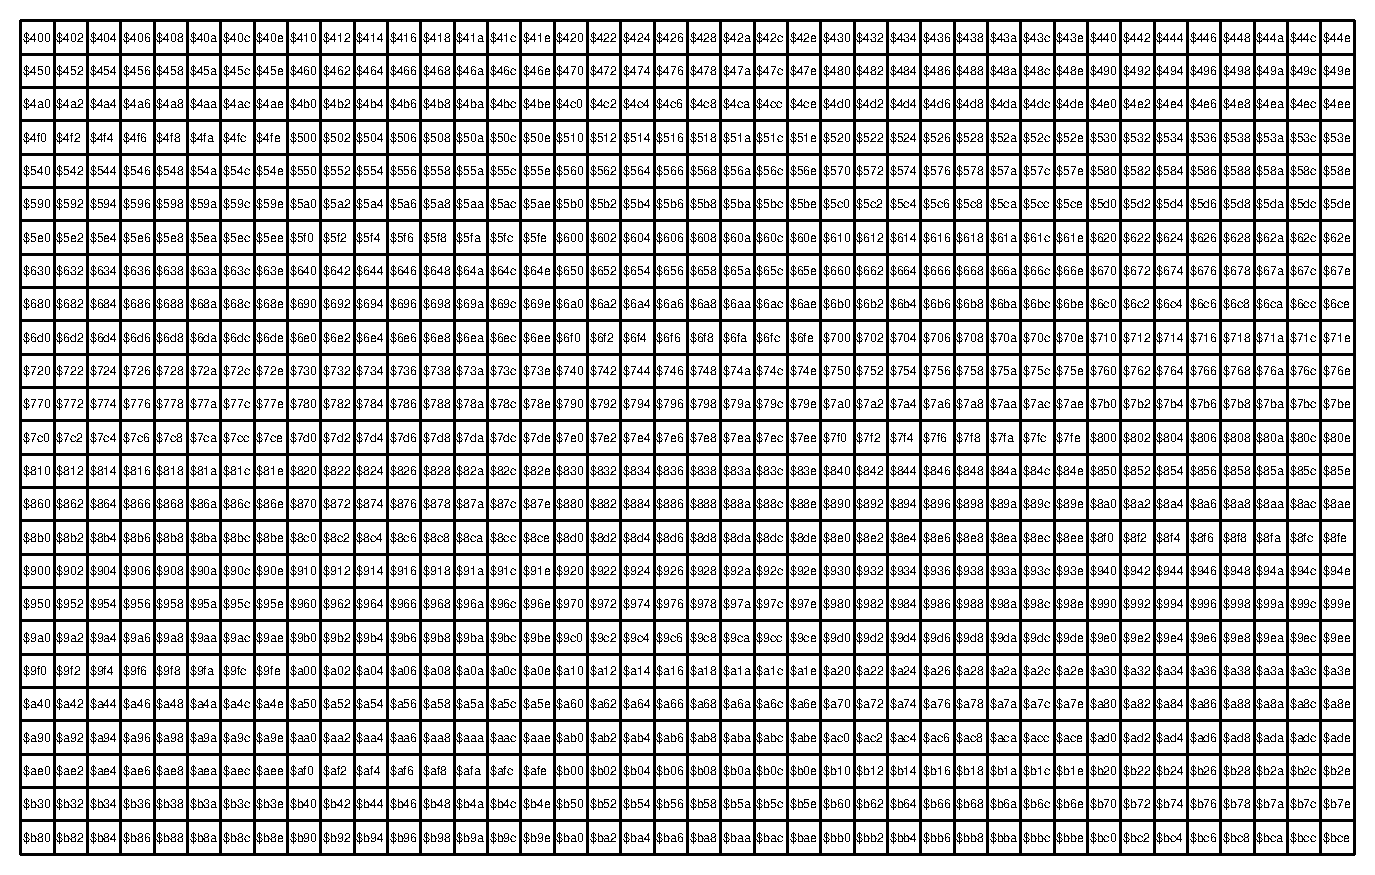
\includegraphics[width=\linewidth]{images/illustrations/screen-40x25-addresses16-80.pdf}

Het is mogelijk om Super-Uitgebreide Attribuutmodus te gebruiken vanuit C65-modus, door het scherm op 80 kolommen in te stellen, omdat de C65-ROM 2 KB reserveert voor zowel het schermgeheugen als het kleurengeheugen, en automatisch \$D058 en \$D059 op de juiste waarde zet voor 40$\times$2 = 80 bytes per schermregel. De gebruiker hoeft elk tekenpaar slechts als één Super-Uitgebreid Attribuutteken te behandelen en Super-Uitgebreide Attribuutmodus in te schakelen, zoals hierboven beschreven.

Omdat er paren van kleurengeheugen- en schermgeheugenbytes worden gebruikt om elk teken te definiëren, moet voorzichtig te werk worden gegaan bij het initialiseren en bewerken van het scherm. Een goede aanpak is om de tekstkleur op zwart in te stellen (kleurcode 0) en vervolgens het scherm te vullen met @-tekens, omdat dat tekencode 0 is. Vervolgens zijn er verschillende manieren om het scherm te bewerken. U kunt het normale PRINT-commando gebruiken en zorgvuldig tekenreeksen samenstellen die de juiste waarden in elk scherm- en kleurenbytepaar schrijven. Een andere aanpak is om de BANK- en POKE-commando's te gebruiken om de inhoud van het schermgeheugen en kleurengeheugen direct te instellen.

Het beheren van een scherm in Super-Uitgebreide Attribuutmodus op deze manier met BASIC 65 is natuurlijk eerder een noodoplossing en wordt alleen voorgesteld als een relatief eenvoudige manier om te beginnen met experimenteren. U wilt bijna zeker snel overschakelen op aangepaste schermverwerkingscode, het liefst in assembleertaal, om schermen in Super-Uitgebreide Attribuutmodus te bewerken. De aanpak met BASIC 65 kan echter behoorlijk krachtig zijn, omdat het bestaande scrollen van het scherm en andere bewerkingen beschikbaar blijven.

XXX Voorbeeldprogramma

De volgende beschrijvingen gaan ervan uit dat u een van de hierboven beschreven methoden heeft geïmplementeerd om het schermgeheugen en kleurengeheugen in te stellen.

\subsection{Volkleur-tekstmodus (256 kleuren per teken) (FCM)}

In de normale VIC-II/III-tekstmodus wordt één byte gebruikt voor elke pixelrij in een teken. Ter herinnering aan de werking van die modes: in hoge-resolutiemodus is elke pixel ofwel de achtergrond- ofwel de voorgrondkleur, gebaseerd op één bit in de byte. Kleurenmodus gebruikt twee bits om tussen vier mogelijke kleuren te kiezen, maar omdat er nog steeds slechts 8 bits beschikbaar zijn om elke rij van 8 pixels te beschrijven, heeft elk pixelpaar dezelfde kleur. De volkleur-tekstmodus van de VIC-IV schaft deze beperkingen op en maakt het mogelijk om elke pixel van een teken te kiezen uit 256 kleuren van de primaire of alternatieve paletbank, zonder horizontale resolutie op te offeren.

Hiertoe heeft elk teken nu 64 bytes aan gegevens nodig. Het adres van de gegevens is 64 $\times$ het tekennummer, ongeacht het adres van de tekenset. FCM hoort normaal gesproken te worden gebruikt met Super-Uitgebreide Attribuutmodus (SEAM), zodat meer dan 256 unieke tekens kunnen worden aangesproken. Omdat SEAM de keuze van 8.192 unieke tekens mogelijk maakt, kunnen FCM-tekengegevens overal in de eerste 512 KB chip-RAM worden geplaatst (let er echter op dat de meeste MEGA65-modellen slechts 384 KB chip-RAM hebben).

Let erop dat pixelwaarde \$ff niet direct de bijbehorende kleurcode selecteert. In plaats daarvan selecteert deze de kleurcode die is gedefinieerd door het kleurengeheugen.

\subsection{Nibble-kleuren-tekstmodus (16 kleuren per teken) (NCM)}

De Nibble-kleuren-modus (NCM) voor tekst lijkt op Volkleur-tekstmodus, met als verschil dat elke byte gegevens twee pixels beschrijft met elk 4 bits. Dit maakt NCM uniek, omdat de tekens 16 pixels breed zullen zijn in plaats van de gebruikelijke 8 pixels. Dit kan worden gebruikt om kleurrijke weergaven te maken, zonder zoveel geheugen te gebruiken als FCM, omdat er minder tekens nodig zijn om het scherm te bedekken. In tegenstelling tot de multicolourmodus (MCM) van de VIC-II heeft deze modus geen verlies van horizontale resolutie tot gevolg.

Bij NCM komen de onderste vier bits van de pixelkleur van de bovenste of onderste vier bits van de pixelgegevens. De bovenste vier bits van de kleurcode komen van de kleurengeheugengegevens van het weergegeven teken. Hierdoor is het mogelijk om alle paletingangen in NCM te gebruiken, hoewel de beperking van 16 kleuren per teken blijft bestaan. Vergelijkbaar met het gedrag van FCM selecteert pixelgegevenswaarde \$f de pixelkleur die is ingesteld in het kleurengeheugen.

Een verder voordeel van NCM is dat het minder buscycli per pixel gebruikt dan FCM, omdat er minder tekengegevens-ophaalbewerkingen per rasterlijn hoeven plaats te vinden. Samen met de verminderde geheugenbehoeften maakt dit NCM bijzonder geschikt voor het maken van kleurrijke grafische lagen. Hiermee kan de VIC-IV arcade-achtige weergaven met meer kleuren tonen dan bij veel 16-bits computers.


XXX

\subsection{Alphablending / Anti-aliasing}

De VIC-IV ondersteunt het mengen van tekens met de achtergrondkleur, waardoor effecten zoals anti-aliased lettertype-weergave mogelijk zijn. Het mengen is mogelijk op per-teken-basis. Het wordt ingeschakeld voor een specifiek teken als aan de volgende voorwaarden wordt voldaan:
\begin{enumerate}
  \item Het {\em ALPHAEN}-signaal is ingesteld in bit 7 van \$D054.  \item Het {\em CHR16}-signaal is ingesteld in bit 0 van \$D054 om Super-Uitgebreide Attribuutmodus (SEAM) in te schakelen.  \item Volkleur-tekstmodus (FCM) is ingeschakeld voor het teken.
\end{enumerate}
Indien alphablending is ingeschakeld voor een teken, worden de 8-bit pixelwaarden behandeld als alphawaarden in plaats van paletindices. De werkelijke pixelkleur wordt bepaald door de achtergrondkleur te mengen met de voorgrondkleur van het teken zoals gedefinieerd in het kleurengeheugen. Een alphawaarde van 0 staat voor volledige transparantie, waarbij alleen de achtergrondkleur van die pixel wordt weergegeven.

Merk op dat de alphablending alleen wordt toegepast tussen de achtergrondkleur en de voorgrondkleur van het teken. Dit betekent dat tekens achter het huidige teken feitelijk niet zichtbaar zullen zijn (tekenlagen kunnen worden samengesteld via GOTOX-herpositionering). Programmeurs moeten er echter van uitgaan dat het mengen met eerdere lagen in een toekomstige implementatie zal worden ondersteund. Om problemen met een dergelijke wijziging te voorkomen, plaatst u geen tekens achter een teken waarvoor alphablending is ingeschakeld.



\subsection{Tekens omdraaien}

XXX

\subsection{Variabele-breedte lettertypen}

Er zijn 4 bits waarmee pixels van de rechterrand van tekens kunnen worden weggesneden wanneer deze worden weergegeven. Dit heeft het effect dat tekens smaller worden. Dit kan nuttig zijn voor aantrekkelijkere tekstweergave, waarbij smallere tekens zoals ``i'' minder ruimte innemen dan bredere tekens zoals ``m'', zonder dat een bitmapdisplay nodig is. Deze functie kan worden gebruikt om variabele-breedte tekstweergave zeer efficiënt te maken, zowel wat betreft geheugengebruik als verwerkingstijd.

Deze functie kan worden gecombineerd met de volkleur-tekstmodus, de alfa-blendmodus en de 4-bits-per-pixel-modus om tekens mogelijk te maken met 15 intensiteitsniveaus tussen de achtergrond- en voorgrondkleur, en tot 16 pixels breed. Bovendien kan het GOTO-bit worden gebruikt om negatieve kerning toe te passen, zodat tekenparen zoals A en T geen overbodige witruimte tussen zich hebben wanneer ze naast elkaar worden afgedrukt. Het zorgvuldig gebruik van deze functies kan leiden tot indrukwekkende tekstweergave, vergelijkbaar met die op moderne 32-bits en 64-bits systemen, maar die nog steeds efficiënt genoeg is om te worden geïmplementeerd op een relatief beperkt systeem zoals de MEGA65. De presentatiesoftware ``MegaWAT!?’’'' voor de MEGA65 maakt gebruik van verschillende van deze functies om zijn aantrekkelijke, antialiased proportionele tekstweergave op dia's te produceren.

XXX MEGAWat!?!-screenshot

XXX Voorbeeldprogramma

\subsection{Raster Re-write Buffer}

Als het GOTO-bit is gezet voor een teken in Super-Uitgebreide Attribuutmodus, wordt in plaats van het teken te tekenen de positie op de rasterlijn teruggedraaid (of vooruitgeschoven) naar de pixelpositie die is opgegeven in de onderste 10 bits van de schermgeheugenbytes. Als het vertical flip-bit is gezet, heeft dit de alternatieve betekenis dat de achtergrondkleur niet wordt getekend. Deze combinatie kan worden gebruikt om tekstmateriaal over ander tekstmateriaal te plaatsen, wat een grove aanvulling vormt op de 8 hardware-sprites. De hoeveelheid materiaal is alleen beperkt door de rastertijd van de VIC-IV. Enige experimentatie is vereist om te bepalen hoeveel er in PAL- en NTSC-modus kan worden bereikt.

Als het GOTO-bit is gezet voor een teken en de tekenbreedte-verminderingsbits ook zijn gezet, worden deze geïnterpreteerd als een Y-offset die wordt opgeteld bij het tekengeheugenadres, maar alleen in Volkleurmodus. Instellen van Y=1 zorgt ervoor dat de tekendata worden opgehaald van 8 bytes verder, d.w.z. de eerste rij tekendata komt van het adres waar normaal de tweede rij tekendata zou worden opgehaald. Voor hogere waarden worden de tekendata opgehaald van verderop in de tekens. Door tekens zorgvuldig in het geheugen te rangschikken, kan deze functie worden gebruikt om vrije verticale positionering van soft sprites mogelijk te maken, zonder dat de tekendata hoeven te worden gekopieerd.

Als het GOTO-bit is gezet voor een teken en het Nybl Colour Mode (NCM)-bit ook is gezet, wordt het tweede kleurengeheugenbyte voor dat teken gebruikt om de \index{Rijmasker}rijmasker-bits in te stellen. Voor elk bit dat in het rijmasker is gezet, wordt de overeenkomstige rij tekens in de regel niet weergegeven. Dit kan worden gecombineerd met de Y-offsetfunctie om effectief een soepele verticale schuifregeling per teken mogelijk te maken.

De mogelijkheid om meerdere lagen tekst en grafisch materiaal te tekenen is zeer krachtig. Dit kan bijvoorbeeld worden gebruikt om meerdere overlappende lagen van apart schuifbare grafische elementen te bieden. Dit geeft veel van de voordelen van bitplane-gebaseerde playfields op andere computers, zoals de Amiga, maar zonder de nadelen van bitplanes.

Een goede introductie van de Raster Re-write Buffer en het gebruik ervan is te vinden in deze video:

\url{https://www.youtube.com/watch?v=00bm5uBeBos&feature=youtu.be}

Een belangrijk aspect van de RRB is dat de VIC-IV alleen de tekendata weergeeft die zich links van, en inclusief, het laatst getekende teken bevindt. Dit betekent dat wanneer u de GOTO-token gebruikt om meerdere lagen grafisch materiaal te overschrijven, u ofwel moet zorgen dat de laatste laag tot aan de rechterrand van het scherm reikt, ofwel een GOTO-token moet toevoegen dat de renderpositie naar de rechterrand van het scherm verplaatst.


XXX Voorbeeldprogramma

\section{Sprites}

\subsection{VIC-II/III-spritebesturing}

De besturing van sprites voor C64 / VIC-II/III-compatibiliteit is ongewijzigd ten opzichte van de C64. De enige praktische verschillen zijn zeer gering. In het bijzonder gebruikt de VIC-IV een ringbuffer voor de gegevens van elke sprite bij het renderen van een rasterlijn. Dit betekent dat een sprite meerdere keren per rasterlijn kan worden weergegeven, wat horizontale multiplexing mogelijk maakt.

\subsection{Uitgebreide sprite-afbeeldingssets}

Op de VIC-II en VIC-III moeten alle sprites hun afbeeldingsdata op een bepaald moment uit één enkel 16KB-geheugengebied halen. Dit beperkt het aantal verschillende sprite-afbeeldingen tot 256, omdat elke sprite-afbeelding 64 bytes in beslag neemt. In de praktijk moet hetzelfde 16KB-geheugengebied ook bitmap-, tekst- of bitplanedata bevatten, wat het aantal sprite-afbeeldingen dat tegelijk kan worden gebruikt aanzienlijk beperkt.

De VIC-IV heft deze beperking op doordat spritedata overal in het geheugen kunnen worden geplaatst, zij het nog steeds op 64-byte-grenzen. Dit wordt gedaan door het SPRPTR16-signaal in te stellen (bit 7, \$D06E, decimaal 53358), wat de VIC-IV vertelt dat er twee bytes per spritepointer in plaats van één moeten worden verwacht. Deze adressen zijn dan absolute adressen en negeren de 16KB VIC-II-bankselectielogica. Er zijn dus 16 bytes nodig in plaats van 8 bytes. De lijst met pointers kan ook overal in het geheugen worden geplaatst door de SPRPTRADR (\$D06C -- \$D06D, 53356 -- 53357 decimaal) en SPRPTRBNK-signalen (bits 0 -- 6, \$D06E, 53358 decimaal) in te stellen. Hierdoor kunnen spritedata overal in de eerste 4MB RAM worden geplaatst en de spritepointerlijst overal in de eerste 8MB RAM. Let op dat typische installaties van de VIC-IV slechts 384KB aangesloten RAM hebben, zodat deze beperkingen geen praktisch effect hebben. De bovenste bits van het SPRPTRBNK-signaal moeten echter op nul worden gezet om problemen met voorwaartse compatibiliteit te voorkomen.

Een reden voor ondersteuning van meer sprite-afbeeldingen is dat sprites op de VIC-IV meer dan één 64-byte-afbeeldingsslot kunnen vereisen. Het inschakelen van de modus voor extra-brede sprites betekent bijvoorbeeld dat een sprite 8$\times$21 = 168 bytes nodig heeft en dus vier VIC-II-stijl 64-byte-spriteafbeeldingsslots inneemt. Wanneer sprites met variabele hoogte worden gebruikt, kan dit oplopen tot 8$\times$255 = 2.040 bytes per sprite.

\subsection{Variabele spritegrootte}

Sprites kunnen met de VIC-IV een van drie breedtes hebben:

\begin{enumerate}
\item Normale VIC-II-breedte (24 pixels breed).\item Extra Breed, waarbij 64 bits (8 bytes) data per rasterlijn worden gebruikt in plaats van de 24 van de VIC-II. Dit resulteert in sprites die 64 pixels breed zijn, tenzij Volkleur-spritemodus is geselecteerd voor een sprite, in welk geval de sprite 64 bits $\div$ 4 bits per pixel = 16 pixels breed zal zijn.\item Tegelmodus, waarbij de sprite wordt herhaald getekend tot het einde van de rasterlijn. \\  Tegelmodus moet normaal gesproken alleen worden gebruikt met extra-brede sprites, omdat het tegelen altijd plaatsvindt met 64 bits spritedata per regel. Het inschakelen van tegelmodus met normale 24 bits brede mono- of multicolour-spritedata tekent 2 en 2/3 rijen spritedata als één regel, zelfs als de sprite niet in extra-brede modus staat, wat tot verwarrende weergave leidt.
\end{enumerate}

Om een sprite 64 pixels breed te maken (of 16 pixels als Volkleur-spritemodus is ingeschakeld), zet u het overeenkomstige bit voor de sprite in het SPRX64EN-register op (\$D057, 53335 decimaal). Het inschakelen van Volkleurmodus voor een sprite schakelt impliciet de uitgebreide breedtemodus in en zorgt ervoor dat deze sprites 16 pixels breed zijn.

Op vergelijkbare wijze kunnen sprites diverse hoogtes hebben: sprites zijn ofwel 21 pixels hoog zoals bij de VIC-II, ofwel, als het overeenkomstige bit voor de sprite is ingeschakeld in het SPRHGTEN-signaal (\$D055, 53333 decimaal), heeft die sprite de hoogte in pixels die is ingesteld in het SPRHGT-register (\$D056, 53334 decimaal), van 0 tot 255. Let op dat alle sprites met SPRHGTEN ingeschakeld dezelfde hoogte delen. Een sprite kan altijd de onderkant van zijn afbeeldingsdata transparant laten.

Om tegelmodus in te schakelen voor een sprite, zet u het bijbehorende bit van SPRTILEN. Voor sprites 0 tot en met 3 zet u bits 4 tot en met 7 van \$D04D (53325 decimaal). Voor sprites 4 tot en met 7 zet u bits 4 tot en met 7 van \$D04F (55327 decimaal).

\subsection{Variabele sprite-resolutie}

Standaard hebben sprites dezelfde resolutie als op de VIC-II, oftewel elke sprite-pixel is twee fysieke pixels breed en hoog. Het is echter mogelijk om sprites de native resolutie te laten gebruiken, waarbij sprite-pixels één fysiek pixel breed en/of hoog zijn. Dit wordt bereikt door het relevante bit voor de sprite in het SPRENV400-register (\$D076, 53366 decimaal) te zetten, zodat de verticale resolutie per sprite wordt vergroot. De horizontale resolutie van alle sprites is ofwel de normale VIC-II-resolutie, of wanneer het SPR640-signaal is gezet (bit 4 van \$D054, 53332 decimaal), hebben sprites dezelfde horizontale resolutie als de fysieke pixels van het beeldscherm.

\subsection{Sprite-paletbank}

De VIC-IV heeft vier paletbanken, in vergelijking met de enkele paletbank van de VIC-III. De VIC-IV maakt het mogelijk om afzonderlijke paletbanken te selecteren voor bitmap-/tekstgraphics en voor sprites. Dit maakt het eenvoudig om zeer kleurrijke beeldschermen te creëren, waarbij sprites andere kleuren hebben dan de rest van het beeldscherm, of om paletanimatie te gebruiken voor interessante visuele effecten in sprites, zonder het palet dat door andere elementen van het beeldscherm wordt gebruikt te verstoren.

De sprite-paletbank wordt geselecteerd door het SPRPALSEL-signaal in bits 2 en 3 van het register \$D070 (53360 decimaal) te zetten. Het is mogelijk om deze op dezelfde bank als de bitmap-/tekstweergave in te stellen, of om een andere paletbank te selecteren. De selectie van de paletbank wordt onmiddellijk van kracht. Vergeet niet dat u, om een palet te kunnen wijzigen, het palet ook in het bereik van de paletbankregisters op \$D100 -- \$D3FF moet plaatsen door het MAPEDPAL-signaal in bits 6 en 7 van \$D070 te zetten.

\subsection{Vollekleuren-spritemodus}

Naast de monochrome en multicolour-modi ondersteunt de VIC-IV een nieuwe vollekleuren-spritemodus. In deze modus worden vier bits gebruikt om elke sprite-pixel te coderen. In tegenstelling tot de multicolour-modus, waarin paren van bits paren van pixels coderen, behouden de pixels in de vollekleurenmodus hun normale horizontale resolutie. De kleur nul wordt als transparant beschouwd. Indien u zwart wilt gebruiken in een vollekleurensprite, moet u de paletbank die voor sprites is geselecteerd zodanig configureren dat een van de 15 kleuren voor de betreffende sprite de kleur zwart codeert.

De vollekleuren-spritemodus kan per sprite worden geselecteerd door het bijbehorende bit in het SPR16EN-register (\$D06B, 53355 decimaal) te zetten.

Om de acht sprites elk 15 unieke kleuren te laten hebben, wordt de spritekleur weergegeven met behulp van de paletingang die overeenkomt met: $spritenummer \times 16 + nibblewaarde$, waarbij $spritenummer$ het nummer van de sprite is (van 0 tot en met 7) en $nibblewaarde$ de waarde is van het halfbyte dat de spritegegevens voor de pixel bevat. Indien bovendien de bitplane-modus voor deze sprite is ingeschakeld, wordt 128 opgeteld bij de kleurwaarde, waardoor het eenvoudig wordt om tussen twee kleurenschema's voor een gegeven sprite te schakelen door slechts één bit in het SPRBPMEN-register te wijzigen.

Omdat de vollekleuren-spritemodus vier bits per pixel vereist, zijn sprites slechts zes pixels breed, tenzij extra-breed voor een sprite is ingeschakeld, in welk geval de sprite 16 pixels breed is. Tegelmodus kan gecombineerd worden met de vollekleuren-spritemodus, en heeft dan tot gevolg dat de 16 vollekleuren-pixels van de sprite worden herhaald tot aan het einde van de rasterlijn.

Het volgende BASIC-programma tekent een vollekleurensprite in C64- of C65-modus:

\begin{screencode}
10 PRINT CHR$(147)
20 REM C65-/C64-MODUS DETECTEREN
30 IF PEEK(53272) AND 32 THEN GOTO 100
40 POKE 53295,ASC("G"):POKE 53295,ASC("S")
100 REM Sprite instellen
110 AD=4096                         :REM $1000-spriteadres
120 TC=10                           :REM transparante kleur
130 SPR=PEEK(53356)+PEEK(53357)*256 :REM sprite-tabeladres ophalen
140 POKE SPR,AD/64                  :REM spriteadres instellen
150 FOR I=AD TO AD+168              :REM sprite met TC wissen
160 POKE I,TC+TC*16                 :REM een byte = 2 pixels
170 NEXT
180 POKE 53287,TC                   :REM transparante kleur instellen
190 POKE 53248,100                  :REM sprite op 100,100 zetten...
200 POKE 53249,100                  :REM op het scherm op 100,100
210 POKE 53355,1                    :REM sprite 0 16-kleurig maken
220 POKE 53335,1                    :REM sprite 0 16X4-bits laten gebruiken
230 POKE 53269,1                    :REM sprite 0 inschakelen
240 GOSUB 900                       :REM meerkleurensprite lezen
250 END

900 REM Sprite uit gegevens laden
910 READ N$:IF N$="END" THEN RETURN
920 GOSUB 1000                      :REM regel decoderen
930 GOTO 910

\end{screencode}

\begin{screencode}
1000 REM Tekenreeks van nibbles in N$ op adres AD decoderen
1010 IF LEN(N$)<>16 THEN PRINT "ILLEGAL SPR DATA!":END
1020 FOR I=1 TO 16 STEP 2
1030 N=(ASC(MID$(N$,I,1))-ASC("@"))    :REM hoge nibble
1040 IF N<0 THEN N=TC                  :REM . is transparant
1050 M=(ASC(MID$(N$,I+1,1))-ASC("@"))  :REM lage nibble
1060 IF M<0 THEN M=TC                  :REM . is transparant
1070 POKE AD,(N AND 15)*16 + (M AND 15):REM 2 pixels instellen
1080 AD=AD+1                           :REM AD ophogen
1090 NEXT I
1100 RETURN

1998 REM Spritegegevens
1999 REM . = transparant, @-O = kleuren 0 tot 15
2000 DATA "..AAFF...HHCC..."
2010 DATA ".AAFF.....HHCC.."
2020 DATA "AAFF.......HHCC."
2030 DATA "AFF...@@@...HHC."
2040 DATA "FF..@@GGG@@..HH."
2050 DATA "..@@GGGGGGG@@..."
2060 DATA ".@GGGGGGGGGGG@.."
2070 DATA ".@GGGGGGGGGGG@.."
2080 DATA "@GGG@@GGG@@GGG@."
2090 DATA "@GG@GGGGGGG@GG@."
2100 DATA "@GGGGGGGGGGGGG@."
2110 DATA "@GGGGGBGBGGGGG@."
2120 DATA "@GGGBBBBBBBGGG@."
2130 DATA ".@GGGGBBBGGGG@.."
2140 DATA ".@GGGGGBGGGGG@.."
2150 DATA "..@@GGGGGGG@@..."
2160 DATA "II..@@GGG@@..KK."
2170 DATA "DII...@@@...KKE."
2180 DATA "DDII.......KKEE."
2190 DATA ".DDII.....KKEE.."
2200 DATA "..DDII...KKEE..."
2210 DATA "END"
\end{screencode}
\clearpage

\section{VIC-III errata-niveau}

Er zijn een aantal gevallen waarin de VIC-III-chip in de bekende Commodore 65-prototypen niet overeenkomstig de specificatie functioneert, de specificatie onvoldoende detail bevat en de implementatie opmerkelijk inconsistent is, of het ontwerp zelf gebreken of inconsistenties vertoont. Het standaardgedrag van de VIC-IV is om de VIC-III in deze gevallen zo nauwkeurig mogelijk te emuleren. In sommige gevallen waarin het gedrag van de VIC-III tekortschiet, biedt de VIC-IV verbeterd gedrag, dat door software kan worden geselecteerd met behulp van het HWERRATA-register op \$D08F.

Omdat deze correcties achterwaarts onverenigbaar zijn met de VIC-III en met eerdere versies van de VIC-IV en de MEGA65-core, moet software deze correcties expliciet activeren door het HWERRATA-register te zetten. Dit beschermt software tegen verdere wijzigingen die in toekomstige versies van de MEGA65-core kunnen worden geïntroduceerd. De beginstand van dit register is \$00, wat volledige compatibiliteit met de VIC-III aanvraagt, inclusief het foutieve gedrag. De MEGA65-ROM zal dit register bij het starten van programma's altijd op \$00 laten staan. Een programma kan HWERRATA instellen om een set correcties te activeren die de ontwikkelaar bij het schrijven van het programma kende, en achterwaarts onverenigbare correcties uit te sluiten die in latere versies kunnen worden geïntroduceerd.

Het aanvragen van een errata-niveau activeert alle correcties tot dat niveau. Er is bewust geen mogelijkheid om een niveau aan te vragen en specifieke correcties op lagere niveaus uit te sluiten. U moet uw programma zodanig schrijven dat het alle correcties tot het gevraagde niveau ondersteunt.

In gevallen waarin het activeren van een correctie het gedrag van een heet register wijzigt, zal het instellen van het errata-niveau hete-registerpropagatie {\em{niet}} activeren. Het programma moet de hete-registerpropagatie zelf activeren door een 1 te schrijven naar het HOTREG-register.

De tot nu toe geïmplementeerde errata-niveaus zijn als volgt:

\subsubsection{VIC-III errata-niveaus}

\begin{longtable}{|p{1.5cm}|p{7.1cm}|p{2.5cm}|}
\hhline{---}
{\bf{Niveau}} & {\bf{Gecorrigeerd gedrag}} & {\bf{Ge\"introduceerd in}} \\
\hhline{---}
\endhead
\multicolumn{3}{l@{}}{vervolg \ldots}\\
\endfoot
\hline
\endlastfoot

{\bf{0}} & Geen correcties. Volledig VIC-III-compatibel. & N/A \\

\hline
{\bf{1}} & {\bf{X-scrollpositie verschoven in de H640-modus.}} De VIC-III geeft de X-scrollpositie voor het vloeiend scrollen van tekst (\$D016 XSCL) onjuist weer in de H640-modus. De correctie verschuift de scrollpositie met 1 logische pixel (2 fysieke pixels) naar rechts. Dit wordt pas van kracht na de hot register-propagatie. &v0.96 \\

\hline
{\bf{X}} & {\bf{Gedrag van de busy-vlag van de SD-kaart.}} De busy-vlag van de SD-kaart (bit 1 van \$D680) geeft aan of de SD-kaartcontroller op laag niveau bezig is. Door de toevoeging van de read-ahead-functionaliteit van de SD-kaartcontroller zal oudere software, die erop rekent dat dit bit vrijkomt na voltooiing van een leesbewerking, ten onrechte wachten totdat de volledige read-ahead-sequentie is afgerond. Dit kan er op zijn beurt toe leiden dat software ten onrechte meent dat het lezen van de sector is mislukt vanwege de langere benodigde tijd, of dat een ander leesverzoek niet onmiddellijk kan worden ingediend. Daarom geeft de busy-vlag van de SD-kaart onder dit errata-niveau niet aan of de SD-kaartcontroller een read-ahead-bewerking op de achtergrond voor een sector uitvoert. Op of boven dit errata-niveau wordt deze informatie niet verborgen: bit 0 komt vrij wanneer de gevraagde sector beschikbaar is, maar bit 1 blijft gezet zolang een read-ahead-bewerking doorgaat. &Nog niet geïmplementeerd \\

\end{longtable}


\section{VIC-II / C64-registers}

\setlength{\tabcolsep}{0pt}
\begin{longtable}{|C{12.5mm}|C{12.5mm}|C{12.5mm}|C{12.5mm}|C{12.5mm}|C{12.5mm}|C{12.5mm}|C{12.5mm}|C{12.5mm}|C{12.5mm}|}
\hline
{\bf{HEX}} & {\bf{DEC}} & {\bf{DB7}} & {\bf{DB6}} & {\bf{DB5}} & {\bf{DB4}} & {\bf{DB3}} & {\bf{DB2}} & {\bf{DB1}} & {\bf{DB0}} \\
\hline
\endfirsthead
\multicolumn{3}{l@{}}{\ldots vervolgd}\\
\hline
{\bf{HEX}} & {\bf{DEC}} & {\bf{DB7}} & {\bf{DB6}} & {\bf{DB5}} & {\bf{DB4}} & {\bf{DB3}} & {\bf{DB2}} & {\bf{DB1}} & {\bf{DB0}} \\
\endhead
\multicolumn{3}{l@{}}{vervolgd \ldots}\\
\endfoot
\hline
\endlastfoot
\footnotesize  D000\index{Registers!\$D000} \index{Registers!53248} & \footnotesize 53248 & \multicolumn{8}{c|}{\footnotesize S0X\index{Registers!SNX}}\\
\hline
\footnotesize  D001\index{Registers!\$D001} \index{Registers!53249} & \footnotesize 53249 & \multicolumn{8}{c|}{\footnotesize S0Y\index{Registers!SNY}}\\
\hline
\footnotesize  D002\index{Registers!\$D002} \index{Registers!53250} & \footnotesize 53250 & \multicolumn{8}{c|}{\footnotesize S1X\index{Registers!S1X}}\\
\hline
\footnotesize  D003\index{Registers!\$D003} \index{Registers!53251} & \footnotesize 53251 & \multicolumn{8}{c|}{\footnotesize S1Y\index{Registers!S1Y}}\\
\hline
\footnotesize  D004\index{Registers!\$D004} \index{Registers!53252} & \footnotesize 53252 & \multicolumn{8}{c|}{\footnotesize S2X\index{Registers!S2X}}\\
\hline
\footnotesize  D005\index{Registers!\$D005} \index{Registers!53253} & \footnotesize 53253 & \multicolumn{8}{c|}{\footnotesize S2Y\index{Registers!S2Y}}\\
\hline
\footnotesize  D006\index{Registers!\$D006} \index{Registers!53254} & \footnotesize 53254 & \multicolumn{8}{c|}{\footnotesize S3X\index{Registers!S3X}}\\
\hline
\footnotesize  D007\index{Registers!\$D007} \index{Registers!53255} & \footnotesize 53255 & \multicolumn{8}{c|}{\footnotesize S3Y\index{Registers!S3Y}}\\
\hline
\footnotesize  D008\index{Registers!\$D008} \index{Registers!53256} & \footnotesize 53256 & \multicolumn{8}{c|}{\footnotesize S4X\index{Registers!S4X}}\\
\hline
\footnotesize  D009\index{Registers!\$D009} \index{Registers!53257} & \footnotesize 53257 & \multicolumn{8}{c|}{\footnotesize S4Y\index{Registers!S4Y}}\\
\hline
\footnotesize  D00A\index{Registers!\$D00A} \index{Registers!53258} & \footnotesize 53258 & \multicolumn{8}{c|}{\footnotesize S5X\index{Registers!S5X}}\\
\hline
\footnotesize  D00B\index{Registers!\$D00B} \index{Registers!53259} & \footnotesize 53259 & \multicolumn{8}{c|}{\footnotesize S5Y\index{Registers!S5Y}}\\
\hline
\footnotesize  D00C\index{Registers!\$D00C} \index{Registers!53260} & \footnotesize 53260 & \multicolumn{8}{c|}{\footnotesize S6X\index{Registers!S6X}}\\
\hline
\footnotesize  D00D\index{Registers!\$D00D} \index{Registers!53261} & \footnotesize 53261 & \multicolumn{8}{c|}{\footnotesize S6Y\index{Registers!S6Y}}\\
\hline
\footnotesize  D00E\index{Registers!\$D00E} \index{Registers!53262} & \footnotesize 53262 & \multicolumn{8}{c|}{\footnotesize S7X\index{Registers!S7X}}\\
\hline
\footnotesize  D00F\index{Registers!\$D00F} \index{Registers!53263} & \footnotesize 53263 & \multicolumn{8}{c|}{\footnotesize S7Y\index{Registers!S7Y}}\\
\hline
\footnotesize  D010\index{Registers!\$D010} \index{Registers!53264} & \footnotesize 53264 & \multicolumn{8}{c|}{\footnotesize SXMSB\index{Registers!SXMSB}}\\
\hline
\footnotesize  D011\index{Registers!\$D011} \index{Registers!53265} & \footnotesize 53265 & \footnotesize RC8 & \footnotesize ECM & \footnotesize BMM & \footnotesize BLNK & \footnotesize RSEL & \multicolumn{3}{c|}{\footnotesize YSCL\index{Registers!YSCL}}\\
\hline
\footnotesize  D012\index{Registers!\$D012} \index{Registers!53266} & \footnotesize 53266 & \multicolumn{8}{c|}{\footnotesize RC\index{Registers!RC}}\\
\hline
\footnotesize  D013\index{Registers!\$D013} \index{Registers!53267} & \footnotesize 53267 & \multicolumn{8}{c|}{\footnotesize LPX\index{Registers!LPX}}\\
\hline
\footnotesize  D014\index{Registers!\$D014} \index{Registers!53268} & \footnotesize 53268 & \multicolumn{8}{c|}{\footnotesize LPY\index{Registers!LPY}}\\
\hline
\footnotesize  D015\index{Registers!\$D015} \index{Registers!53269} & \footnotesize 53269 & \multicolumn{8}{c|}{\footnotesize SE\index{Registers!SE}}\\
\hline
\footnotesize  D016\index{Registers!\$D016} \index{Registers!53270} & \footnotesize 53270 & \multicolumn{2}{c|}{\footnotesize --}& \footnotesize RST & \footnotesize MCM & \footnotesize CSEL & \multicolumn{3}{c|}{\footnotesize XSCL\index{Registers!XSCL}}\\
\hline
\footnotesize  D017\index{Registers!\$D017} \index{Registers!53271} & \footnotesize 53271 & \multicolumn{8}{c|}{\footnotesize SEXY\index{Registers!SEXY}}\\
\hline
\footnotesize  D018\index{Registers!\$D018} \index{Registers!53272} & \footnotesize 53272 & \multicolumn{4}{c|}{\footnotesize VS\index{Registers!VS}}& \multicolumn{3}{c|}{\footnotesize CB\index{Registers!CB}}& \footnotesize -- \\
\hline
\footnotesize  D019\index{Registers!\$D019} \index{Registers!53273} & \footnotesize 53273 & \multicolumn{4}{c|}{\footnotesize --}& \footnotesize ILP & \footnotesize ISSC & \footnotesize ISBC & \footnotesize RIRQ \\
\hline
\footnotesize  D01A\index{Registers!\$D01A} \index{Registers!53274} & \footnotesize 53274 & \multicolumn{5}{c|}{\footnotesize --}& \footnotesize MISSC & \footnotesize MISBC & \footnotesize MRIRQ \\
\hline
\footnotesize  D01B\index{Registers!\$D01B} \index{Registers!53275} & \footnotesize 53275 & \multicolumn{8}{c|}{\footnotesize BSP\index{Registers!BSP}}\\
\hline
\footnotesize  D01C\index{Registers!\$D01C} \index{Registers!53276} & \footnotesize 53276 & \multicolumn{8}{c|}{\footnotesize SCM\index{Registers!SCM}}\\
\hline
\footnotesize  D01D\index{Registers!\$D01D} \index{Registers!53277} & \footnotesize 53277 & \multicolumn{8}{c|}{\footnotesize SEXX\index{Registers!SEXX}}\\
\hline
\footnotesize  D01E\index{Registers!\$D01E} \index{Registers!53278} & \footnotesize 53278 & \multicolumn{8}{c|}{\footnotesize SSC\index{Registers!SSC}}\\
\hline
\footnotesize  D01F\index{Registers!\$D01F} \index{Registers!53279} & \footnotesize 53279 & \multicolumn{8}{c|}{\footnotesize SBC\index{Registers!SBC}}\\
\hline
\footnotesize  D020\index{Registers!\$D020} \index{Registers!53280} & \footnotesize 53280 & \multicolumn{4}{c|}{\footnotesize --}& \multicolumn{4}{c|}{\footnotesize BORDERCOL\index{Registers!BORDERCOL}}\\
\hline
\footnotesize  D021\index{Registers!\$D021} \index{Registers!53281} & \footnotesize 53281 & \multicolumn{4}{c|}{\footnotesize --}& \multicolumn{4}{c|}{\footnotesize SCREENCOL\index{Registers!SCREENCOL}}\\
\hline
\footnotesize  D022\index{Registers!\$D022} \index{Registers!53282} & \footnotesize 53282 & \multicolumn{4}{c|}{\footnotesize --}& \multicolumn{4}{c|}{\footnotesize MC1\index{Registers!MC1}}\\
\hline
\footnotesize  D023\index{Registers!\$D023} \index{Registers!53283} & \footnotesize 53283 & \multicolumn{4}{c|}{\footnotesize --}& \multicolumn{4}{c|}{\footnotesize MC2\index{Registers!MC2}}\\
\hline
\footnotesize  D024\index{Registers!\$D024} \index{Registers!53284} & \footnotesize 53284 & \multicolumn{4}{c|}{\footnotesize --}& \multicolumn{4}{c|}{\footnotesize MC3\index{Registers!MC3}}\\
\hline
\footnotesize  D025\index{Registers!\$D025} \index{Registers!53285} & \footnotesize 53285 & \multicolumn{8}{c|}{\footnotesize SPRMC0\index{Registers!SPRMC0}}\\
\hline
\footnotesize  D026\index{Registers!\$D026} \index{Registers!53286} & \footnotesize 53286 & \multicolumn{8}{c|}{\footnotesize SPRMC1\index{Registers!SPRMC1}}\\
\hline
\footnotesize  D027\index{Registers!\$D027} \index{Registers!53287} & \footnotesize 53287 & \multicolumn{8}{c|}{\footnotesize SPR0COL\index{Registers!SPRNCOL}}\\
\hline
\footnotesize  D028\index{Registers!\$D028} \index{Registers!53288} & \footnotesize 53288 & \multicolumn{8}{c|}{\footnotesize SPR1COL\index{Registers!SPR1COL}}\\
\hline
\footnotesize  D029\index{Registers!\$D029} \index{Registers!53289} & \footnotesize 53289 & \multicolumn{8}{c|}{\footnotesize SPR2COL\index{Registers!SPR2COL}}\\
\hline
\footnotesize  D02A\index{Registers!\$D02A} \index{Registers!53290} & \footnotesize 53290 & \multicolumn{8}{c|}{\footnotesize SPR3COL\index{Registers!SPR3COL}}\\
\hline
\footnotesize  D02B\index{Registers!\$D02B} \index{Registers!53291} & \footnotesize 53291 & \multicolumn{8}{c|}{\footnotesize SPR4COL\index{Registers!SPR4COL}}\\
\hline
\footnotesize  D02C\index{Registers!\$D02C} \index{Registers!53292} & \footnotesize 53292 & \multicolumn{8}{c|}{\footnotesize SPR5COL\index{Registers!SPR5COL}}\\
\hline
\footnotesize  D02D\index{Registers!\$D02D} \index{Registers!53293} & \footnotesize 53293 & \multicolumn{8}{c|}{\footnotesize SPR6COL\index{Registers!SPR6COL}}\\
\hline
\footnotesize  D02E\index{Registers!\$D02E} \index{Registers!53294} & \footnotesize 53294 & \multicolumn{8}{c|}{\footnotesize SPR7COL\index{Registers!SPR7COL}}\\
\hline
\footnotesize  D02F\index{Registers!\$D02F} \index{Registers!53295} & \footnotesize 53295 & \multicolumn{8}{c|}{\footnotesize KEY\index{Registers!KEY}}\\
\hline
\footnotesize  D030\index{Registers!\$D030} \index{Registers!53296} & \footnotesize 53296 & \multicolumn{7}{c|}{\footnotesize --}& \footnotesize C128\-FAST \\
\hline
\end{longtable}
\begin{itemize}
\item{\bf{BLNK}\index{Registers!BLNK}} Weergave inschakelen: 0 = weergave uitschakelen, 1 = weergave inschakelen
\item{\bf{BMM}\index{Registers!BMM}} Bitmapmodus
\item{\bf{BORDERCOL}\index{Registers!BORDERCOL}} Randkleur van het scherm (16 kleuren)
\item{\bf{BSP}\index{Registers!BSP}} Bitstelling sprite-/achtergrondprioriteit
\item{\bf{C128FAST}\index{Registers!C128FAST}} 2 MHz-selectie (voor C128 2 MHz-emulatie)
\item{\bf{CB}\index{Registers!CB}} Adreslocatie van de tekenset (× 1 KiB)
\item{\bf{CSEL}\index{Registers!CSEL}} 38/40-kolommenselectie
\item{\bf{ECM}\index{Registers!ECM}} Uitgebreide achtergrondmodus
\item{\bf{ILP}\index{Registers!ILP}} Lichtpen indicator of bevestiging
\item{\bf{ISBC}\index{Registers!ISBC}} Sprite-/bitmapbotsing indicator of bevestiging
\item{\bf{ISSC}\index{Registers!ISSC}} Sprite-/spritebotsing indicator of bevestiging
\item{\bf{KEY}\index{Registers!KEY}} \$00 en dan \$00 schrijven om C64/VIC-II I/O-registers in te schakelen
\item{\bf{LPX}\index{Registers!LPX}} Grove horizontale bundelpositie (was lichtpen X)
\item{\bf{LPY}\index{Registers!LPY}} Grove verticale bundelpositie (was lichtpen Y)
\item{\bf{MC1}\index{Registers!MC1}} Multikleur 1 (16 kleuren)
\item{\bf{MC2}\index{Registers!MC2}} Multikleur 2 (16 kleuren)
\item{\bf{MC3}\index{Registers!MC3}} Multikleur 3 (16 kleuren)
\item{\bf{MCM}\index{Registers!MCM}} Multikleurmodus
\item{\bf{MISBC}\index{Registers!MISBC}} Masker sprite-/bitmapbotsing IRQ
\item{\bf{MISSC}\index{Registers!MISSC}} Masker sprite-/spritebotsing IRQ
\item{\bf{MRIRQ}\index{Registers!MRIRQ}} Masker rasterIRQ
\item{\bf{RC}\index{Registers!RC}} Rastervergelijking bits 0 tot 7
\item{\bf{RC8}\index{Registers!RC8}} Rastervergelijking bit 8
\item{\bf{RIRQ}\index{Registers!RIRQ}} Rastervergelijking indicator of bevestiging
\item{\bf{RSEL}\index{Registers!RSEL}} 24/25-rijselectie
\item{\bf{RST}\index{Registers!RST}} Schakelt de video-uitvoer op de MAX Machine(tm) VIC-II 6566 uit. Wordt genegeerd op normale C64-computers en de MEGA65
\item{\bf{SBC}\index{Registers!SBC}} Indicatiebits voor sprite/voorgrondbotsing
\item{\bf{SCM}\index{Registers!SCM}} Inschakelbits voor de sprite-multikleur
\item{\bf{SCREENCOL}\index{Registers!SCREENCOL}} Schermkleur (16 kleuren)
\item{\bf{SE}\index{Registers!SE}} Inschakelbits voor sprites
\item{\bf{SEXX}\index{Registers!SEXX}} Inschakelbits voor horizontale sprite-vergroting
\item{\bf{SEXY}\index{Registers!SEXY}} Inschakelbits voor verticale sprite-vergroting
\item{\bf{SNX}\index{Registers!SNX}} Horizontale positie van sprite N
\item{\bf{SNY}\index{Registers!SNY}} Verticale positie van sprite N
\item{\bf{SPRMC0}\index{Registers!SPRMC0}} Sprite-multikleur 0
\item{\bf{SPRMC1}\index{Registers!SPRMC1}} Sprite-multikleur 1
\item{\bf{SPRNCOL}\index{Registers!SPRNCOL}} Kleur van sprite N / transparantiekleur van de sprite in 16-kleurenmodus (lagere nibble)
\item{\bf{SSC}\index{Registers!SSC}} Indicatiebits voor sprite/spritebotsing
\item{\bf{SXMSB}\index{Registers!SXMSB}} MSB's van de horizontale sprite-positie
\item{\bf{VS}\index{Registers!VS}} Schermadres ($\times$ 1KiB)
\item{\bf{XSCL}\index{Registers!XSCL}} Horizontaal vloeiend scrollen
\item{\bf{YSCL}\index{Registers!YSCL}} 24/25 verticaal vloeiend scrollen
\end{itemize}


\section{VIC-III / C65-registers}

\setlength{\tabcolsep}{0pt}
\begin{longtable}{|C{12.5mm}|C{12.5mm}|C{12.5mm}|C{12.5mm}|C{12.5mm}|C{12.5mm}|C{12.5mm}|C{12.5mm}|C{12.5mm}|C{12.5mm}|}
\hline
{\bf{HEX}} & {\bf{DEC}} & {\bf{DB7}} & {\bf{DB6}} & {\bf{DB5}} & {\bf{DB4}} & {\bf{DB3}} & {\bf{DB2}} & {\bf{DB1}} & {\bf{DB0}} \\
\hline
\endfirsthead
\multicolumn{3}{l@{}}{\ldots vervolgd}\\
\hline
{\bf{HEX}} & {\bf{DEC}} & {\bf{DB7}} & {\bf{DB6}} & {\bf{DB5}} & {\bf{DB4}} & {\bf{DB3}} & {\bf{DB2}} & {\bf{DB1}} & {\bf{DB0}} \\
\endhead
\multicolumn{3}{l@{}}{vervolgd \ldots}\\
\endfoot
\hline
\endlastfoot
\footnotesize  D020\index{Registers!\$D020} \index{Registers!53280} & \footnotesize 53280 & \multicolumn{8}{c|}{\footnotesize BORDERCOL\index{Registers!BORDERCOL}}\\
\hline
\footnotesize  D021\index{Registers!\$D021} \index{Registers!53281} & \footnotesize 53281 & \multicolumn{8}{c|}{\footnotesize SCREENCOL\index{Registers!SCREENCOL}}\\
\hline
\footnotesize  D022\index{Registers!\$D022} \index{Registers!53282} & \footnotesize 53282 & \multicolumn{8}{c|}{\footnotesize MC1\index{Registers!MC1}}\\
\hline
\footnotesize  D023\index{Registers!\$D023} \index{Registers!53283} & \footnotesize 53283 & \multicolumn{8}{c|}{\footnotesize MC2\index{Registers!MC2}}\\
\hline
\footnotesize  D024\index{Registers!\$D024} \index{Registers!53284} & \footnotesize 53284 & \multicolumn{8}{c|}{\footnotesize MC3\index{Registers!MC3}}\\
\hline
\footnotesize  D025\index{Registers!\$D025} \index{Registers!53285} & \footnotesize 53285 & \multicolumn{8}{c|}{\footnotesize SPRMC0\index{Registers!SPRMC0}}\\
\hline
\footnotesize  D026\index{Registers!\$D026} \index{Registers!53286} & \footnotesize 53286 & \multicolumn{8}{c|}{\footnotesize SPRMC1\index{Registers!SPRMC1}}\\
\hline
\footnotesize  D02F\index{Registers!\$D02F} \index{Registers!53295} & \footnotesize 53295 & \multicolumn{8}{c|}{\footnotesize KEY\index{Registers!KEY}}\\
\hline
\footnotesize  D030\index{Registers!\$D030} \index{Registers!53296} & \footnotesize 53296 & \footnotesize ROME & \footnotesize CROM9 & \footnotesize ROMC & \footnotesize ROMA & \footnotesize ROM8 & \footnotesize PAL & \footnotesize EXTSYNC & \footnotesize CRAM2K \\
\hline
\footnotesize  D031\index{Registers!\$D031} \index{Registers!53297} & \footnotesize 53297 & \footnotesize H640 & \footnotesize FAST & \footnotesize ATTR & \footnotesize BPM & \footnotesize V400 & \footnotesize H1280 & \footnotesize MONO & \footnotesize INT \\
\hline
\footnotesize  D032\index{Registers!\$D032} \index{Registers!53298} & \footnotesize 53298 & \multicolumn{8}{c|}{\footnotesize BPENABLE\index{Registers!BPENABLE}}\\
\hline
\footnotesize  D033\index{Registers!\$D033} \index{Registers!53299} & \footnotesize 53299 & \multicolumn{3}{c|}{\footnotesize B0ADODD\index{Registers!BXADODD}}& \footnotesize -- & \multicolumn{3}{c|}{\footnotesize B0ADEVN\index{Registers!BXADEVN}}& \footnotesize -- \\
\hline
\footnotesize  D034\index{Registers!\$D034} \index{Registers!53300} & \footnotesize 53300 & \multicolumn{3}{c|}{\footnotesize B1ADODD\index{Registers!BYADODD}}& \footnotesize -- & \multicolumn{3}{c|}{\footnotesize B1ADEVN\index{Registers!BYADEVN}}& \footnotesize -- \\
\hline
\footnotesize  D035\index{Registers!\$D035} \index{Registers!53301} & \footnotesize 53301 & \multicolumn{3}{c|}{\footnotesize B2ADODD\index{Registers!B2ADODD}}& \footnotesize -- & \multicolumn{3}{c|}{\footnotesize B2ADEVN\index{Registers!B2ADEVN}}& \footnotesize -- \\
\hline
\footnotesize  D036\index{Registers!\$D036} \index{Registers!53302} & \footnotesize 53302 & \multicolumn{3}{c|}{\footnotesize B3ADODD\index{Registers!B3ADODD}}& \footnotesize -- & \multicolumn{3}{c|}{\footnotesize B3ADEVN\index{Registers!B3ADEVN}}& \footnotesize -- \\
\hline
\footnotesize  D037\index{Registers!\$D037} \index{Registers!53303} & \footnotesize 53303 & \multicolumn{3}{c|}{\footnotesize B4ADODD\index{Registers!B4ADODD}}& \footnotesize -- & \multicolumn{3}{c|}{\footnotesize B4ADEVN\index{Registers!B4ADEVN}}& \footnotesize -- \\
\hline
\footnotesize  D038\index{Registers!\$D038} \index{Registers!53304} & \footnotesize 53304 & \multicolumn{3}{c|}{\footnotesize B5ADODD\index{Registers!B5ADODD}}& \footnotesize -- & \multicolumn{3}{c|}{\footnotesize B5ADEVN\index{Registers!B5ADEVN}}& \footnotesize -- \\
\hline
\footnotesize  D039\index{Registers!\$D039} \index{Registers!53305} & \footnotesize 53305 & \multicolumn{3}{c|}{\footnotesize B6ADODD\index{Registers!B6ADODD}}& \footnotesize -- & \multicolumn{3}{c|}{\footnotesize B6ADEVN\index{Registers!B6ADEVN}}& \footnotesize -- \\
\hline
\footnotesize  D03A\index{Registers!\$D03A} \index{Registers!53306} & \footnotesize 53306 & \multicolumn{3}{c|}{\footnotesize B7ADODD\index{Registers!B7ADODD}}& \footnotesize -- & \multicolumn{3}{c|}{\footnotesize B7ADEVN\index{Registers!B7ADEVN}}& \footnotesize -- \\
\hline
\footnotesize  D03B\index{Registers!\$D03B} \index{Registers!53307} & \footnotesize 53307 & \multicolumn{8}{c|}{\footnotesize BPCOMP\index{Registers!BPCOMP}}\\
\hline
\footnotesize  D03C\index{Registers!\$D03C} \index{Registers!53308} & \footnotesize 53308 & \multicolumn{8}{c|}{\footnotesize BPX\index{Registers!BPX}}\\
\hline
\footnotesize  D03D\index{Registers!\$D03D} \index{Registers!53309} & \footnotesize 53309 & \multicolumn{8}{c|}{\footnotesize BPY\index{Registers!BPY}}\\
\hline
\footnotesize  D03E\index{Registers!\$D03E} \index{Registers!53310} & \footnotesize 53310 & \multicolumn{8}{c|}{\footnotesize HPOS\index{Registers!HPOS}}\\
\hline
\footnotesize  D03F\index{Registers!\$D03F} \index{Registers!53311} & \footnotesize 53311 & \multicolumn{8}{c|}{\footnotesize VPOS\index{Registers!VPOS}}\\
\hline
\footnotesize  D040\index{Registers!\$D040} \index{Registers!53312} & \footnotesize 53312 & \multicolumn{8}{c|}{\footnotesize B0PIX\index{Registers!BNPIX}}\\
\hline
\footnotesize  D041\index{Registers!\$D041} \index{Registers!53313} & \footnotesize 53313 & \multicolumn{8}{c|}{\footnotesize B1PIX\index{Registers!B1PIX}}\\
\hline
\footnotesize  D042\index{Registers!\$D042} \index{Registers!53314} & \footnotesize 53314 & \multicolumn{8}{c|}{\footnotesize B2PIX\index{Registers!B2PIX}}\\
\hline
\footnotesize  D043\index{Registers!\$D043} \index{Registers!53315} & \footnotesize 53315 & \multicolumn{8}{c|}{\footnotesize B3PIX\index{Registers!B3PIX}}\\
\hline
\footnotesize  D044\index{Registers!\$D044} \index{Registers!53316} & \footnotesize 53316 & \multicolumn{8}{c|}{\footnotesize B4PIX\index{Registers!B4PIX}}\\
\hline
\footnotesize  D045\index{Registers!\$D045} \index{Registers!53317} & \footnotesize 53317 & \multicolumn{8}{c|}{\footnotesize B5PIX\index{Registers!B5PIX}}\\
\hline
\footnotesize  D046\index{Registers!\$D046} \index{Registers!53318} & \footnotesize 53318 & \multicolumn{8}{c|}{\footnotesize B6PIX\index{Registers!B6PIX}}\\
\hline
\footnotesize  D047\index{Registers!\$D047} \index{Registers!53319} & \footnotesize 53319 & \multicolumn{8}{c|}{\footnotesize B7PIX\index{Registers!B7PIX}}\\
\hline
\footnotesize  D100 -- D1FF\index{Registers!\$D100 -- \$D1FF} \index{Registers!53504 -- 53759} & \footnotesize 53504 -- 53759 & \multicolumn{8}{c|}{\footnotesize PALRED\index{Registers!PALRED}}\\
\hline
\footnotesize  D200 -- D2FF\index{Registers!\$D200 -- \$D2FF} \index{Registers!53760 -- 54015} & \footnotesize 53760 -- 54015 & \multicolumn{8}{c|}{\footnotesize PALGREEN\index{Registers!PALGREEN}}\\
\hline
\footnotesize  D300 -- D3FF\index{Registers!\$D300 -- \$D3FF} \index{Registers!54016 -- 54271} & \footnotesize 54016 -- 54271 & \multicolumn{8}{c|}{\footnotesize PALBLUE\index{Registers!PALBLUE}}\\
\hline
\end{longtable}
\begin{itemize}
\item{\bf{ATTR}\index{Registers!ATTR}} Uitgebreide attributen en 8-bits kleuringangen inschakelen
\item{\bf{BNPIX}\index{Registers!BNPIX}} Display Address Translater (DAT) Bitplane N-poort
\item{\bf{BORDERCOL}\index{Registers!BORDERCOL}} Weergaverandkleur (256 kleuren)
\item{\bf{BPCOMP}\index{Registers!BPCOMP}} Complement-vlaggen voor bitplanes
\item{\bf{BPENABLE}\index{Registers!BPENABLE}} Inschakelbits voor bitplanes
\item{\bf{BPM}\index{Registers!BPM}} Bitplane-modus
\item{\bf{BPX}\index{Registers!BPX}} Bitplane X
\item{\bf{BPY}\index{Registers!BPY}} Bitplane Y
\item{\bf{BXADEVN}\index{Registers!BXADEVN}} Even rijen van even Bitplane X-adres[15:13] (voor v200 wordt de even rij tweemaal getekend)
\item{\bf{BXADODD}\index{Registers!BXADODD}} Oneven rijen van even Bitplane X-adres[15:13] (wordt alleen gebruikt in de v400-modus)
\item{\bf{BYADEVN}\index{Registers!BYADEVN}} Even rijen van oneven Bitplane Y-adres[15:13] (+64KB) (voor v200 wordt de even rij tweemaal getekend)
\item{\bf{BYADODD}\index{Registers!BYADODD}} Oneven rijen van oneven Bitplane Y-adres[15:13] (+64KB) (wordt alleen gebruikt in de v400-modus)
\item{\bf{CRAM2K}\index{Registers!CRAM2K}} Mapt de 2e KB van het kleurengeheugen \@ \$DC00-\$DFFF
\item{\bf{CROM9}\index{Registers!CROM9}} Selecteert tussen de C64- en C65-tekenset (niet geïmplementeerd)
\item{\bf{EXTSYNC}\index{Registers!EXTSYNC}} Externe videosynchronisatie inschakelen (genlock-ingang)
\item{\bf{FAST}\index{Registers!FAST}} C65 FAST-modus inschakelen ($\sim$3.5MHz)
\item{\bf{H1280}\index{Registers!H1280}} 1280 horizontale pixels inschakelen (niet geïmplementeerd, schakelt PALEMU uit)
\item{\bf{H640}\index{Registers!H640}} C64 640 horizontale pixels / 80-kolommenmodus inschakelen
\item{\bf{HPOS}\index{Registers!HPOS}} Bitplane X-offset
\item{\bf{INT}\index{Registers!INT}} Interlaced modus van de VIC-III inschakelen
\item{\bf{KEY}\index{Registers!KEY}} \$A5 en dan \$96 schrijven om de C65/VIC-III I/O-registers in te schakelen
\item{\bf{MC1}\index{Registers!MC1}} Multikleur 1 (256 kleuren)
\item{\bf{MC2}\index{Registers!MC2}} Multikleur 2 (256 kleuren)
\item{\bf{MC3}\index{Registers!MC3}} Multikleur 3 (256 kleuren)
\item{\bf{MONO}\index{Registers!MONO}} VIC-III MONO-composietvideo-uitvoer inschakelen (kleur indien uitgeschakeld)
\item{\bf{PAL}\index{Registers!PAL}} Gebruikt ingangen van het PALETTE ROM (0) of het RAM (1) voor kleuren 0 - 15
\item{\bf{PALBLUE}\index{Registers!PALBLUE}} Blauwe paletwaarden (omgekeerde nibble-volgorde)
\item{\bf{PALGREEN}\index{Registers!PALGREEN}} Groene paletwaarden (omgekeerde nibble-volgorde)
\item{\bf{PALRED}\index{Registers!PALRED}} Rode paletwaarden (omgekeerde nibble-volgorde)
\item{\bf{ROM8}\index{Registers!ROM8}} Mapt de C65-ROM \@ \$8000
\item{\bf{ROMA}\index{Registers!ROMA}} Mapt de C65-ROM \@ \$A000
\item{\bf{ROMC}\index{Registers!ROMC}} Mapt de C65-ROM \@ \$C000
\item{\bf{ROME}\index{Registers!ROME}} Mapt de C65-ROM \@ \$E000
\item{\bf{SCREENCOL}\index{Registers!SCREENCOL}} Schermkleur (256 kleuren)
\item{\bf{SPRMC0}\index{Registers!SPRMC0}} Sprite-multikleur 0 (8-bits voor selectie van elke paletkleur)
\item{\bf{SPRMC1}\index{Registers!SPRMC1}} Sprite-multikleur 1 (8-bits voor selectie van elke paletkleur)
\item{\bf{V400}\index{Registers!V400}} 400 verticale pixels inschakelen (schakelt PALEMU uit)
\item{\bf{VPOS}\index{Registers!VPOS}} Bitplane Y-offset
\end{itemize}


\section{VIC-IV / MEGA65-specifieke registers}

\setlength{\tabcolsep}{0pt}
\begin{longtable}{|C{12.5mm}|C{12.5mm}|C{12.5mm}|C{12.5mm}|C{12.5mm}|C{12.5mm}|C{12.5mm}|C{12.5mm}|C{12.5mm}|C{12.5mm}|}
\hline
{\bf{HEX}} & {\bf{DEC}} & {\bf{DB7}} & {\bf{DB6}} & {\bf{DB5}} & {\bf{DB4}} & {\bf{DB3}} & {\bf{DB2}} & {\bf{DB1}} & {\bf{DB0}} \\
\hline
\endfirsthead
\multicolumn{3}{l@{}}{\ldots vervolgd}\\
\hline
{\bf{HEX}} & {\bf{DEC}} & {\bf{DB7}} & {\bf{DB6}} & {\bf{DB5}} & {\bf{DB4}} & {\bf{DB3}} & {\bf{DB2}} & {\bf{DB1}} & {\bf{DB0}} \\
\endhead
\multicolumn{3}{l@{}}{vervolgd \ldots}\\
\endfoot
\hline
\endlastfoot
\footnotesize  D020\index{Registers!\$D020} \index{Registers!53280} & \footnotesize 53280 & \multicolumn{8}{c|}{\footnotesize BORDERCOL\index{Registers!BORDERCOL}}\\
\hline
\footnotesize  D021\index{Registers!\$D021} \index{Registers!53281} & \footnotesize 53281 & \multicolumn{8}{c|}{\footnotesize SCREENCOL\index{Registers!SCREENCOL}}\\
\hline
\footnotesize  D022\index{Registers!\$D022} \index{Registers!53282} & \footnotesize 53282 & \multicolumn{8}{c|}{\footnotesize MC1\index{Registers!MC1}}\\
\hline
\footnotesize  D023\index{Registers!\$D023} \index{Registers!53283} & \footnotesize 53283 & \multicolumn{8}{c|}{\footnotesize MC2\index{Registers!MC2}}\\
\hline
\footnotesize  D024\index{Registers!\$D024} \index{Registers!53284} & \footnotesize 53284 & \multicolumn{8}{c|}{\footnotesize MC3\index{Registers!MC3}}\\
\hline
\footnotesize  D025\index{Registers!\$D025} \index{Registers!53285} & \footnotesize 53285 & \multicolumn{8}{c|}{\footnotesize SPRMC0\index{Registers!SPRMC0}}\\
\hline
\footnotesize  D026\index{Registers!\$D026} \index{Registers!53286} & \footnotesize 53286 & \multicolumn{8}{c|}{\footnotesize SPRMC1\index{Registers!SPRMC1}}\\
\hline
\footnotesize  D02F\index{Registers!\$D02F} \index{Registers!53295} & \footnotesize 53295 & \multicolumn{8}{c|}{\footnotesize KEY\index{Registers!KEY}}\\
\hline
\footnotesize  D048\index{Registers!\$D048} \index{Registers!53320} & \footnotesize 53320 & \multicolumn{8}{c|}{\footnotesize TBDRPOS\index{Registers!TBDRPOS}}\\
\hline
\footnotesize  D049\index{Registers!\$D049} \index{Registers!53321} & \footnotesize 53321 & \multicolumn{4}{c|}{\footnotesize SPRBPMEN\index{Registers!SPRBPMEN}}& \multicolumn{4}{c|}{\footnotesize TBDRPOS\index{Registers!TBDRPOS}}\\
\hline
\footnotesize  D04A\index{Registers!\$D04A} \index{Registers!53322} & \footnotesize 53322 & \multicolumn{8}{c|}{\footnotesize BBDRPOS\index{Registers!BBDRPOS}}\\
\hline
\footnotesize  D04B\index{Registers!\$D04B} \index{Registers!53323} & \footnotesize 53323 & \multicolumn{4}{c|}{\footnotesize SPRBPMEN\index{Registers!SPRBPMEN}}& \multicolumn{4}{c|}{\footnotesize BBDRPOS\index{Registers!BBDRPOS}}\\
\hline
\footnotesize  D04C\index{Registers!\$D04C} \index{Registers!53324} & \footnotesize 53324 & \multicolumn{8}{c|}{\footnotesize TEXTXPOS\index{Registers!TEXTXPOS}}\\
\hline
\footnotesize  D04D\index{Registers!\$D04D} \index{Registers!53325} & \footnotesize 53325 & \multicolumn{4}{c|}{\footnotesize SPRTILEN\index{Registers!SPRTILEN}}& \multicolumn{4}{c|}{\footnotesize TEXTXPOS\index{Registers!TEXTXPOS}}\\
\hline
\footnotesize  D04E\index{Registers!\$D04E} \index{Registers!53326} & \footnotesize 53326 & \multicolumn{8}{c|}{\footnotesize TEXTYPOS\index{Registers!TEXTYPOS}}\\
\hline
\footnotesize  D04F\index{Registers!\$D04F} \index{Registers!53327} & \footnotesize 53327 & \multicolumn{4}{c|}{\footnotesize SPRTILEN\index{Registers!SPRTILEN}}& \multicolumn{4}{c|}{\footnotesize TEXTYPOS\index{Registers!TEXTYPOS}}\\
\hline
\footnotesize  D050\index{Registers!\$D050} \index{Registers!53328} & \footnotesize 53328 & \multicolumn{8}{c|}{\footnotesize XPOSLSB\index{Registers!XPOSLSB}}\\
\hline
\footnotesize  D051\index{Registers!\$D051} \index{Registers!53329} & \footnotesize 53329 & \footnotesize NORRDEL & \footnotesize DBLRR & \multicolumn{6}{c|}{\footnotesize XPOSMSB\index{Registers!XPOSMSB}}\\
\hline
\footnotesize  D052\index{Registers!\$D052} \index{Registers!53330} & \footnotesize 53330 & \multicolumn{8}{c|}{\footnotesize FNRASTERLSB\index{Registers!FNRASTERLSB}}\\
\hline
\footnotesize  D053\index{Registers!\$D053} \index{Registers!53331} & \footnotesize 53331 & \footnotesize FNRST & \footnotesize SHDEMU & \footnotesize UPSCALE & \footnotesize BOLDISALT & \multicolumn{4}{c|}{\footnotesize FN\-RASTER\-MSB\index{Registers!FNRASTERMSB}}\\
\hline
\footnotesize  D054\index{Registers!\$D054} \index{Registers!53332} & \footnotesize 53332 & \footnotesize ALPHEN & \footnotesize VFAST & \footnotesize PALEMU & \footnotesize SPR\-H640 & \footnotesize SMTH & \footnotesize FCLRHI & \footnotesize FCLRLO & \footnotesize CHR16 \\
\hline
\footnotesize  D055\index{Registers!\$D055} \index{Registers!53333} & \footnotesize 53333 & \multicolumn{8}{c|}{\footnotesize SPRHGTEN\index{Registers!SPRHGTEN}}\\
\hline
\footnotesize  D056\index{Registers!\$D056} \index{Registers!53334} & \footnotesize 53334 & \multicolumn{8}{c|}{\footnotesize SPRHGHT\index{Registers!SPRHGHT}}\\
\hline
\footnotesize  D057\index{Registers!\$D057} \index{Registers!53335} & \footnotesize 53335 & \multicolumn{8}{c|}{\footnotesize SPRX64EN\index{Registers!SPRX64EN}}\\
\hline
\footnotesize  D058\index{Registers!\$D058} \index{Registers!53336} & \footnotesize 53336 & \multicolumn{8}{c|}{\footnotesize LINESTEPLSB\index{Registers!LINESTEPLSB}}\\
\hline
\footnotesize  D059\index{Registers!\$D059} \index{Registers!53337} & \footnotesize 53337 & \multicolumn{8}{c|}{\footnotesize LINESTEPMSB\index{Registers!LINESTEPMSB}}\\
\hline
\footnotesize  D05A\index{Registers!\$D05A} \index{Registers!53338} & \footnotesize 53338 & \multicolumn{8}{c|}{\footnotesize CHRXSCL\index{Registers!CHRXSCL}}\\
\hline
\footnotesize  D05B\index{Registers!\$D05B} \index{Registers!53339} & \footnotesize 53339 & \multicolumn{8}{c|}{\footnotesize CHRYSCL\index{Registers!CHRYSCL}}\\
\hline
\footnotesize  D05C\index{Registers!\$D05C} \index{Registers!53340} & \footnotesize 53340 & \multicolumn{8}{c|}{\footnotesize SDBDRWD\-LSB\index{Registers!SDBDRWDLSB}}\\
\hline
\footnotesize  D05D\index{Registers!\$D05D} \index{Registers!53341} & \footnotesize 53341 & \footnotesize HOTREG & \footnotesize RST\-DELEN & \multicolumn{6}{c|}{\footnotesize SDBDRWD\-MSB\index{Registers!SDBDRWDMSB}}\\
\hline
\footnotesize  D05E\index{Registers!\$D05E} \index{Registers!53342} & \footnotesize 53342 & \multicolumn{8}{c|}{\footnotesize CHRCOUNT\index{Registers!CHRCOUNT}}\\
\hline
\footnotesize  D05F\index{Registers!\$D05F} \index{Registers!53343} & \footnotesize 53343 & \multicolumn{8}{c|}{\footnotesize SPRXSMSBS\index{Registers!SPRXSMSBS}}\\
\hline
\footnotesize  D060\index{Registers!\$D060} \index{Registers!53344} & \footnotesize 53344 & \multicolumn{8}{c|}{\footnotesize SCRNPTRLSB\index{Registers!SCRNPTRLSB}}\\
\hline
\footnotesize  D061\index{Registers!\$D061} \index{Registers!53345} & \footnotesize 53345 & \multicolumn{8}{c|}{\footnotesize SCRNPTRMSB\index{Registers!SCRNPTRMSB}}\\
\hline
\footnotesize  D062\index{Registers!\$D062} \index{Registers!53346} & \footnotesize 53346 & \multicolumn{8}{c|}{\footnotesize SCRNPTRBNK\index{Registers!SCRNPTRBNK}}\\
\hline
\footnotesize  D063\index{Registers!\$D063} \index{Registers!53347} & \footnotesize 53347 & \footnotesize EXGLYPH & \footnotesize FCOLMCM & \multicolumn{2}{c|}{\footnotesize CHRCOUNT\index{Registers!CHRCOUNT}}& \multicolumn{4}{c|}{\footnotesize SCRNPTRMB\index{Registers!SCRNPTRMB}}\\
\hline
\footnotesize  D064\index{Registers!\$D064} \index{Registers!53348} & \footnotesize 53348 & \multicolumn{8}{c|}{\footnotesize COLPTRLSB\index{Registers!COLPTRLSB}}\\
\hline
\footnotesize  D065\index{Registers!\$D065} \index{Registers!53349} & \footnotesize 53349 & \multicolumn{8}{c|}{\footnotesize COLPTRMSB\index{Registers!COLPTRMSB}}\\
\hline
\footnotesize  D068\index{Registers!\$D068} \index{Registers!53352} & \footnotesize 53352 & \multicolumn{8}{c|}{\footnotesize CHARPTRLSB\index{Registers!CHARPTRLSB}}\\
\hline
\footnotesize  D069\index{Registers!\$D069} \index{Registers!53353} & \footnotesize 53353 & \multicolumn{8}{c|}{\footnotesize CHARPTRMSB\index{Registers!CHARPTRMSB}}\\
\hline
\footnotesize  D06A\index{Registers!\$D06A} \index{Registers!53354} & \footnotesize 53354 & \multicolumn{8}{c|}{\footnotesize CHARPTRBNK\index{Registers!CHARPTRBNK}}\\
\hline
\footnotesize  D06B\index{Registers!\$D06B} \index{Registers!53355} & \footnotesize 53355 & \multicolumn{8}{c|}{\footnotesize SPR16EN\index{Registers!SPR16EN}}\\
\hline
\footnotesize  D06C\index{Registers!\$D06C} \index{Registers!53356} & \footnotesize 53356 & \multicolumn{8}{c|}{\footnotesize SPRPTRADRLSB\index{Registers!SPRPTRADRLSB}}\\
\hline
\footnotesize  D06D\index{Registers!\$D06D} \index{Registers!53357} & \footnotesize 53357 & \multicolumn{8}{c|}{\footnotesize SPRPTRADRMSB\index{Registers!SPRPTRADRMSB}}\\
\hline
\footnotesize  D06E\index{Registers!\$D06E} \index{Registers!53358} & \footnotesize 53358 & \footnotesize SPR\-PTR16 & \multicolumn{7}{c|}{\footnotesize SPRPTRBNK\index{Registers!SPRPTRBNK}}\\
\hline
\footnotesize  D06F\index{Registers!\$D06F} \index{Registers!53359} & \footnotesize 53359 & \footnotesize PALNTSC & \footnotesize VGAHDTV & \multicolumn{6}{c|}{\footnotesize RASLINE0\index{Registers!RASLINE0}}\\
\hline
\footnotesize  D070\index{Registers!\$D070} \index{Registers!53360} & \footnotesize 53360 & \multicolumn{2}{c|}{\footnotesize MAPEDPAL\index{Registers!MAPEDPAL}}& \multicolumn{2}{c|}{\footnotesize BTPALSEL\index{Registers!BTPALSEL}}& \multicolumn{2}{c|}{\footnotesize SPRPALSEL\index{Registers!SPRPALSEL}}& \multicolumn{2}{c|}{\footnotesize ABTPALSEL\index{Registers!ABTPALSEL}}\\
\hline
\footnotesize  D071\index{Registers!\$D071} \index{Registers!53361} & \footnotesize 53361 & \multicolumn{8}{c|}{\footnotesize BP16ENS\index{Registers!BP16ENS}}\\
\hline
\footnotesize  D072\index{Registers!\$D072} \index{Registers!53362} & \footnotesize 53362 & \multicolumn{8}{c|}{\footnotesize SPRYADJ\index{Registers!SPRYADJ}}\\
\hline
\footnotesize  D073\index{Registers!\$D073} \index{Registers!53363} & \footnotesize 53363 & \multicolumn{4}{c|}{\footnotesize RASTERHEIGHT\index{Registers!RASTERHEIGHT}}& \multicolumn{4}{c|}{\footnotesize ALPHADELAY\index{Registers!ALPHADELAY}}\\
\hline
\footnotesize  D074\index{Registers!\$D074} \index{Registers!53364} & \footnotesize 53364 & \multicolumn{8}{c|}{\footnotesize SPRENALPHA\index{Registers!SPRENALPHA}}\\
\hline
\footnotesize  D075\index{Registers!\$D075} \index{Registers!53365} & \footnotesize 53365 & \multicolumn{8}{c|}{\footnotesize SPRALPHAVAL\index{Registers!SPRALPHAVAL}}\\
\hline
\footnotesize  D076\index{Registers!\$D076} \index{Registers!53366} & \footnotesize 53366 & \multicolumn{8}{c|}{\footnotesize SPRENV400\index{Registers!SPRENV400}}\\
\hline
\footnotesize  D077\index{Registers!\$D077} \index{Registers!53367} & \footnotesize 53367 & \multicolumn{8}{c|}{\footnotesize SPRYMSBS\index{Registers!SPRYMSBS}}\\
\hline
\footnotesize  D078\index{Registers!\$D078} \index{Registers!53368} & \footnotesize 53368 & \multicolumn{8}{c|}{\footnotesize SPRYSMSBS\index{Registers!SPRYSMSBS}}\\
\hline
\footnotesize  D079\index{Registers!\$D079} \index{Registers!53369} & \footnotesize 53369 & \multicolumn{8}{c|}{\footnotesize RASCMP\index{Registers!RASCMP}}\\
\hline
\footnotesize  D07A\index{Registers!\$D07A} \index{Registers!53370} & \footnotesize 53370 & \footnotesize FNRST\-CMP & \footnotesize EXTIRQS & \footnotesize NOBUGCOMPAT & \footnotesize CHARY16 & \footnotesize SPTR\-CONT & \multicolumn{3}{c|}{\footnotesize RASCMP\-MSB\index{Registers!RASCMPMSB}}\\
\hline
\footnotesize  D07B\index{Registers!\$D07B} \index{Registers!53371} & \footnotesize 53371 & \multicolumn{8}{c|}{\footnotesize DISP\-ROWS\index{Registers!DISPROWS}}\\
\hline
\footnotesize  D07C\index{Registers!\$D07C} \index{Registers!53372} & \footnotesize 53372 & \multicolumn{2}{c|}{\footnotesize DEBUGC\index{Registers!DEBUGC}}& \footnotesize VSYNCP & \footnotesize HSYNCP & \footnotesize NORRBWRAP & \multicolumn{3}{c|}{\footnotesize BIT\-PBANK\index{Registers!BITPBANK}}\\
\hline
\end{longtable}
\begin{itemize}
\item{\bf{ABTPALSEL}\index{Registers!ABTPALSEL}} Bitmap-/tekstpaletbank van de VIC-IV (alternatief palet)
\item{\bf{ALPHADELAY}\index{Registers!ALPHADELAY}} Alfa-vertraging voor de compositor
\item{\bf{ALPHEN}\index{Registers!ALPHEN}} Alfa-compositor inschakelen
\item{\bf{BBDRPOS}\index{Registers!BBDRPOS}} Positie van de onderrand
\item{\bf{BITPBANK}\index{Registers!BITPBANK}} Bepaalt welke 128KB-bank de bitplanes gebruiken
\item{\bf{BOLDISALT}\index{Registers!BOLDISALT}} Indien gezet, selecteert de BOLD-attribuutbit het alternatieve palet, zonder dat REVERSE eveneens gezet hoeft te worden.
\item{\bf{BORDERCOL}\index{Registers!BORDERCOL}} Weergaverandkleur (256 kleuren)
\item{\bf{BP16ENS}\index{Registers!BP16ENS}} Inschakelvlaggen voor de 16-kleurenbitplanes van de VIC-IV
\item{\bf{BTPALSEL}\index{Registers!BTPALSEL}} Bitmap-/tekstpaletbank
\item{\bf{CHARPTRBNK}\index{Registers!CHARPTRBNK}} Nauwkeurig basisadres van de tekenset (bits 23 - 16)
\item{\bf{CHARPTRLSB}\index{Registers!CHARPTRLSB}} Nauwkeurig basisadres van de tekenset (bits 0 - 7)
\item{\bf{CHARPTRMSB}\index{Registers!CHARPTRMSB}} Nauwkeurig basisadres van de tekenset (bits 15 - 8)
\item{\bf{CHARY16}\index{Registers!CHARY16}} Alternatieve teken-ROM-bank op afwisselende rasterlijnen in V200
\item{\bf{CHR16}\index{Registers!CHR16}} 16-bits teekennummers inschakelen (twee schermbytes per teken)
\item{\bf{CHRCOUNT}\index{Registers!CHRCOUNT}} Aantal weer te geven tekens per rij (LSB)
\item{\bf{CHRXSCL}\index{Registers!CHRXSCL}} Horizontale hardwarematige schaal van de tekstmodus (een honderdtwintigste pixel per pixel)
\item{\bf{CHRYSCL}\index{Registers!CHRYSCL}} Verticale schaling van de tekstmodus (aantal fysieke rasterlijnen per tekstrij)
\item{\bf{COLPTRLSB}\index{Registers!COLPTRLSB}} Basisadres van het kleurengeheugen (bits 0 - 7)
\item{\bf{COLPTRMSB}\index{Registers!COLPTRMSB}} Basisadres van het kleurengeheugen (bits 15 - 8)
\item{\bf{DBLRR}\index{Registers!DBLRR}} Wanneer deze is gezet, wordt de Raster Rewrite Buffer slechts om de tweede rasterlijn bijgewerkt, waardoor de resolutie wordt beperkt tot V200 maar er meer cycli voor Raster-Rewrite-acties overblijven.
\item{\bf{DEBUGC}\index{Registers!DEBUGC}} VIC-IV-debugpixelselectie: het rode (01), groene (10) of blauwe (11) kanaal is zichtbaar in \$D07D
\item{\bf{DISPROWS}\index{Registers!DISPROWS}} Aantal tekstrijen dat moet worden weergegeven
\item{\bf{EXGLYPH}\index{Registers!EXGLYPH}} Haalt full-colour-tekengegevens uit het uitbreidingsgeheugen
\item{\bf{EXTIRQS}\index{Registers!EXTIRQS}} Schakelt extra IRQ-bronnen in, bijv. de raster-X-positie
\item{\bf{FCLRHI}\index{Registers!FCLRHI}} Schakelt de full-colour-modus in voor tekennummers >\$FF
\item{\bf{FCLRLO}\index{Registers!FCLRLO}} Schakelt de full-colour-modus in voor tekennummers <=\$FF
\item{\bf{FCOLMCM}\index{Registers!FCOLMCM}} Schakelt 256 kleuren in de multikleur-tekstmodus in
\item{\bf{FNRASTERLSB}\index{Registers!FNRASTERLSB}} Leest de fysieke rasterpositie
\item{\bf{FNRASTERMSB}\index{Registers!FNRASTERMSB}} Leest de fysieke rasterpositie
\item{\bf{FNRST}\index{Registers!FNRST}} Leest de bron van de rastervergelijking (0=VIC-IV-fijne raster, 1=VIC-II-raster) en levert dezelfde waarde als in FNRSTCMP is ingesteld
\item{\bf{FNRSTCMP}\index{Registers!FNRSTCMP}} De rastervergelijking vindt plaats in fysieke rasterlijnen indien dit bit is gewist, of in VIC-II-lijnen indien het is gezet
\item{\bf{HOTREG}\index{Registers!HOTREG}} Schakelt de VIC-II hot registers in. Wanneer deze zijn ingeschakeld, zorgt het aanraken van veel VIC-II-registers ervoor dat de VIC-IV de weergaveparameters herberekent, zoals randposities en -afmetingen. Het aanraken van registers terwijl deze functie is uitgeschakeld leidt tot een wijziging wanneer deze weer wordt ingeschakeld. Deze waarde op 0 instellen wist de herberekeningsvlag en annuleert de herberekening.
\item{\bf{HSYNCP}\index{Registers!HSYNCP}} hsync-polariteit
\item{\bf{KEY}\index{Registers!KEY}} Schrijf \$47 en dan \$53 om de MEGA65/VIC-IV I/O-registers in te schakelen
\item{\bf{LINESTEPLSB}\index{Registers!LINESTEPLSB}} Aantal bytes waarmee tussen elke tekstrij wordt opgeschoven (LSB)
\item{\bf{LINESTEPMSB}\index{Registers!LINESTEPMSB}} Aantal bytes waarmee tussen elke tekstrij wordt opgeschoven (MSB)
\item{\bf{MAPEDPAL}\index{Registers!MAPEDPAL}} Ingemapte paletbank op \$D100-\$D3FF
\item{\bf{MC1}\index{Registers!MC1}} Multikleur 1 (256 kleuren)
\item{\bf{MC2}\index{Registers!MC2}} Multikleur 2 (256 kleuren)
\item{\bf{MC3}\index{Registers!MC3}} Multikleur 3 (256 kleuren)
\item{\bf{NOBUGCOMPAT}\index{Registers!NOBUGCOMPAT}} *VEROUDERD*, gebruik HWERRATA. Schakelt de VIC-III / C65-bugcompatibiliteitsmodus uit indien deze is gezet
\item{\bf{NORRBWRAP}\index{Registers!NORRBWRAP}} Schakelt de RRB-adreswrap-around uit wanneer deze is gezet
\item{\bf{NORRDEL}\index{Registers!NORRDEL}} Wanneer deze is gewist, wordt dubbelbuffering van de raster rewrite gebruikt
\item{\bf{PALEMU}\index{Registers!PALEMU}} Schakelt PAL-CRT-achtige scanlijn-emulatie in (uitgeschakeld door V400 of H1280)
\item{\bf{PALNTSC}\index{Registers!PALNTSC}} NTSC-emulatiemodus (maximaal raster = 262)
\item{\bf{RASCMP}\index{Registers!RASCMP}} Fysieke rastervergelijkingwaarde die moet worden gebruikt indien FNRSTCMP is gewist
\item{\bf{RASCMPMSB}\index{Registers!RASCMPMSB}} MSB van de rastervergelijkingwaarde
\item{\bf{RASLINE0}\index{Registers!RASLINE0}} Eerste VIC-II-rasterlijn
\item{\bf{RASTERHEIGHT}\index{Registers!RASTERHEIGHT}} Fysieke rasterlijnen per VIC-II-raster (1 tot 16)
\item{\bf{RSTDELEN}\index{Registers!RSTDELEN}} Schakelt de rastervertraging in (vertraagt de rasterteller en interrupts met één regel om aan te sluiten bij de latentie van de uitvoerpipeline)
\item{\bf{SCREENCOL}\index{Registers!SCREENCOL}} Schermkleur (256 kleuren)
\item{\bf{SCRNPTRBNK}\index{Registers!SCRNPTRBNK}} Nauwkeurig basisadres van het scherm-RAM (bits 23 - 16)
\item{\bf{SCRNPTRLSB}\index{Registers!SCRNPTRLSB}} Nauwkeurig basisadres van het scherm-RAM (bits 7 - 0)
\item{\bf{SCRNPTRMB}\index{Registers!SCRNPTRMB}} Nauwkeurig basisadres van het scherm-RAM (bits 27 - 24)
\item{\bf{SCRNPTRMSB}\index{Registers!SCRNPTRMSB}} Nauwkeurig basisadres van het scherm-RAM (bits 15 - 8)
\item{\bf{SDBDRWDLSB}\index{Registers!SDBDRWDLSB}} Breedte van de zijrand (LSB)
\item{\bf{SDBDRWDMSB}\index{Registers!SDBDRWDMSB}} Breedte van de zijrand (MSB)
\item{\bf{SHDEMU}\index{Registers!SHDEMU}} Gesimuleerd schaduwmasker inschakelen (PALEMU moet ook zijn ingeschakeld)
\item{\bf{SMTH}\index{Registers!SMTH}} Horizontale vloeiendheid van de video-uitvoer inschakelen
\item{\bf{SPR16EN}\index{Registers!SPR16EN}} Inschakelbits voor de 16-kleurenmodus van sprites
\item{\bf{SPRALPHAVAL}\index{Registers!SPRALPHAVAL}} Alpha-vermengingswaarde van sprites
\item{\bf{SPRBPMEN}\index{Registers!SPRBPMEN}} Inschakelbits voor de sprite-bitplane-wijzigingsmodus
\item{\bf{SPRENALPHA}\index{Registers!SPRENALPHA}} Alpha-vermenging van sprites inschakelen
\item{\bf{SPRENV400}\index{Registers!SPRENV400}} Inschakelbits voor de V400-modus van sprites
\item{\bf{SPRH640}\index{Registers!SPRH640}} H640-modus van sprites inschakelen
\item{\bf{SPRHGHT}\index{Registers!SPRHGHT}} Grootte van de uitgebreide sprite-hoogte (in sprite-pixels)
\item{\bf{SPRHGTEN}\index{Registers!SPRHGTEN}} Uitgebreide sprite-hoogte inschakelen (één bit per sprite)
\item{\bf{SPRMC0}\index{Registers!SPRMC0}} Sprite-multikleur 0 (8-bits voor de keuze van elke paletkleur)
\item{\bf{SPRMC1}\index{Registers!SPRMC1}} Sprite-multikleur 1 (8-bits voor de keuze van elke paletkleur)
\item{\bf{SPRPALSEL}\index{Registers!SPRPALSEL}} Spritepaletbank
\item{\bf{SPRPTR16}\index{Registers!SPRPTR16}} 16-bits sprite-pointermodus (ermee kunnen sprites op elke 64-bytegrens in chip-RAM worden geplaatst)
\item{\bf{SPRPTRADRLSB}\index{Registers!SPRPTRADRLSB}} Sprite-pointeradres (bits 7 - 0)
\item{\bf{SPRPTRADRMSB}\index{Registers!SPRPTRADRMSB}} Sprite-pointeradres (bits 15 - 8)
\item{\bf{SPRPTRBNK}\index{Registers!SPRPTRBNK}} Sprite-pointeradres (bits 23 - 16)
\item{\bf{SPRTILEN}\index{Registers!SPRTILEN}} Inschakelbits voor horizontale sprite-tegels
\item{\bf{SPRX64EN}\index{Registers!SPRX64EN}} Inschakelbits voor de uitgebreide sprite-breedte (8 bytes per sprite-rij = 64 pixels breed voor normale sprites of 16 pixels breed voor de 16-kleuren-sprite-modus)
\item{\bf{SPRXSMSBS}\index{Registers!SPRXSMSBS}} Super-MSB's van de X-positie van sprites in de H640-modus
\item{\bf{SPRYADJ}\index{Registers!SPRYADJ}} Aanpassing van de Y-positie van sprites
\item{\bf{SPRYMSBS}\index{Registers!SPRYMSBS}} MSB's van de Y-positie van sprites in de V400-modus
\item{\bf{SPRYSMSBS}\index{Registers!SPRYSMSBS}} Super-MSB's van de Y-positie van sprites in de V400-modus
\item{\bf{SPTRCONT}\index{Registers!SPTRCONT}} Bewaakt voortdurend de sprite-pointer zodat de gegevensbron van de sprite kan worden gewijzigd terwijl een sprite wordt getekend
\item{\bf{TBDRPOS}\index{Registers!TBDRPOS}} Positie van de bovenrand
\item{\bf{TEXTXPOS}\index{Registers!TEXTXPOS}} Horizontale positie van de tekengenerator
\item{\bf{TEXTYPOS}\index{Registers!TEXTYPOS}} Verticale positie van de tekengenerator
\item{\bf{UPSCALE}\index{Registers!UPSCALE}} Ingebouwde 720p-upscaler met lage latentie (130 usec) inschakelen
\item{\bf{VFAST}\index{Registers!VFAST}} MEGA65 FAST-modus (40.5MHz)
\item{\bf{VGAHDTV}\index{Registers!VGAHDTV}} Selecteert indien gezet een meer VGA-compatibele modus in plaats van de cyclus-exacte frame-timing van de HDMI/HDTV-VIC-II. Kan helpen om een functioneel beeld op oudere VGA-monitoren te produceren.
\item{\bf{VSYNCP}\index{Registers!VSYNCP}} vsync-polariteit
\item{\bf{XPOSLSB}\index{Registers!XPOSLSB}} Leest de LSB van de horizontale raster-scanpositie
\item{\bf{XPOSMSB}\index{Registers!XPOSMSB}} Leest de MSB van de horizontale raster-scanpositie
\end{itemize}


